\documentclass[a4paper,12pt]{article}

% --- Pakete ---
\usepackage[T1]{fontenc}
\usepackage[utf8]{inputenc}
\usepackage[ngerman]{babel}

\usepackage{geometry}
\geometry{a4paper, margin=2.5cm}

\usepackage{amsmath, amssymb, amsthm}
\usepackage{graphicx}
\usepackage{xcolor}
\usepackage{booktabs}
\usepackage{array}
\usepackage{longtable}
\usepackage{caption}
\usepackage{subcaption}
\usepackage{microtype}
\usepackage{hyperref}
\usepackage{url}

\usepackage{setspace}
\usepackage{enumitem}
\usepackage{fancyhdr}
\usepackage{titlesec}
\usepackage{abstract}
\usepackage{float}
\usepackage{enumitem}


\setlist[itemize]{label=-}

% --- Farben ---
\definecolor{desiblue}{RGB}{30,80,160}
\definecolor{desigold}{RGB}{200,140,30}
\definecolor{desidark}{RGB}{20,30,60}
\definecolor{lightgray}{RGB}{245,245,248}
\definecolor{linkcolor}{RGB}{0,70,140}

% --- Hyperref ---
\hypersetup{
  colorlinks=true,
  linkcolor=linkcolor,
  citecolor=desiblue,
  urlcolor=desiblue,
  pdftitle={DESI: Die größte 3D-Karte des Universums},
  pdfauthor={Stephan Epp},
}

% --- Theorem-Stile ---
\theoremstyle{definition}
\newtheorem{definition}{Definition}[section]
\newtheorem{satz}{Satz}[section]
\newtheorem{lemma}{Lemma}[section]
\newtheorem{korollar}{Korollar}[section]
\newtheorem{proposition}{Proposition}[section]

\theoremstyle{remark}
\newtheorem{bemerkung}{Bemerkung}[section]
\newtheorem{beispiel}{Beispiel}[section]


\title{\textbf{Analyse der kosmologischen Ergebnisse des Dark Energy Spectroscopic Instrument (DESI)}\\
  {\Large Dunkle Energie der Baryonischen Akustischen Oszillationen und der großräumigen Struktur des Universums}}
\date{19. April 2026}

\author{Stephan Epp}

% ============================================================
\begin{document}
% ============================================================

\maketitle

\tableofcontents
\newpage

% ============================================================
\section{Einleitung}
\label{sec:einleitung}
% ============================================================
Das Dark Energy Spectroscopic Instrument (DESI) hat nach Abschluss seines
Fünfjahresprogramms die bislang größte hochauflösende dreidimensionale Karte
des Universums erstellt. Mit über 47 Millionen erfassten Galaxien und Quasaren
sowie über 20 Millionen Sternen in der Milchstraße übertrifft das Ergebnis die
ursprüngliche Zielvorgabe von 34 Millionen Objekten um rund 38\,\%. Die
vorliegende Arbeit analysiert die kosmologischen Messgrößen des Surveys,
insbesondere die Baryonischen Akustischen Oszillationen (BAO) als kosmisches
Standardlineal, den Zustandsparameter der Dunklen Energie $w(z)$, die
Hubble-Spannung sowie die großräumige Struktur des kosmischen Netzes.
Sämtliche Ergebnisse werden formal hergeleitet und durch matplotlib-basierte
Visualisierungen veranschaulicht. Der Ausblick behandelt ausführlich die
Erweiterungsphase DESI~2 (2026--2028) sowie Folgemissionen. Es wird
ausdrücklich darauf hingewiesen, dass die vorliegende Arbeit die
Zahlenwerte und Zeitskalen des Standardmodells der Kosmologie wiedergibt,
ohne damit eine Aussage über ihre Vereinbarkeit mit der biblischen
Schöpfungschronologie zu treffen; dieser Aspekt wird in Abschnitt~\ref{sec:schöpfung}
gesondert diskutiert.

Die großräumige Struktur des Universums -- das sogenannte kosmische Netz aus
Filamenten, Clustern und Voids -- ist eines der direktesten Fenster auf die
fundamentalen Naturgesetze, die den Kosmos formen. Seit den Pionierarbeiten
des \textit{Center for Astrophysics Redshift Survey} (CfA) in den 1980er-Jahren
haben spektroskopische Durchmusterungen einen kontinuierlichen Fortschritt in
der Präzision und Tiefe kosmologischer Messungen ermöglicht \cite{geller1989}.

Das \textbf{Dark Energy Spectroscopic Instrument (DESI)} markiert den bislang
größten Schritt in dieser Entwicklung. Das Instrument operiert am
Nicholas-U.-Mayall-4-Meter-Teleskop auf dem Kitt Peak National Observatory
in Arizona auf einer Höhe von 2\,096\,m über dem Meeresspiegel \cite{desi2016}.
Nach fünf Jahren Betrieb (2021--2026) hat DESI sein Fünfjahresprogramm
abgeschlossen und dabei alle ursprünglichen Zielvorgaben deutlich übertroffen
\cite{desi2024dr1}.

\begin{definition}[DESI-Survey]
  Das DESI Five-Year-Survey bezeichnet das zwischen Mai 2021 und Mai 2026
  durchgeführte spektroskopische Messprogramm, bei dem mit Hilfe von
  5\,000 roboterartig positionierten Glasfasern simultan Spektren von
  Himmelsobjekten aufgenommen wurden, um deren Rotverschiebung und damit
  kosmologische Entfernung zu bestimmen.
\end{definition}

\subsection{Wissenschaftliche Ziele}

Die primären wissenschaftlichen Ziele des DESI-Surveys lassen sich wie folgt
zusammenfassen:

\begin{enumerate}[label=\arabic*.]
  \item \textbf{Messung der Baryonischen Akustischen Oszillationen (BAO)} über
    einen weiten Rotverschiebungsbereich $0{,}1 \leq z \leq 3{,}5$, um die
    kosmologische Expansion mit Prozentgenauigkeit zu verfolgen.
  \item \textbf{Charakterisierung der Dunklen Energie} durch Bestimmung des
    Zustandsparameters $w(z)$ im Rahmen des $w_0 w_a$-CDM-Modells.
  \item \textbf{Präzisionsmessung der Hubble-Konstante $H_0$} und Beitrag zur
    Auflösung der \textit{Hubble-Spannung}.
  \item \textbf{Kartierung der großräumigen Struktur} und Bestimmung der
    Wachstumsrate von Strukturen $f\sigma_8(z)$.
  \item \textbf{Untersuchung der Neutrinomassen} durch kosmologische Constraint-Analysen.
\end{enumerate}

% ============================================================
\section{Das DESI-Instrument}
\label{sec:instrument}
% ============================================================

\subsection{Technische Spezifikationen}

DESI verwendet eine Fokalebene mit \textbf{5\,000 motorisierten Positionierern},
die jeweils eine Glasfaser tragen. Die Positionierer können Himmelsobjekte mit
einer Genauigkeit von $\approx 5\,\mu$m auf der Fokalebene ansteuern, was einem
Winkelfehler von $\approx 0{,}1''$ entspricht \cite{desi2016}. Die Glasfasern
leiten das Licht zu zehn Spektrographen, die einen Wellenlängenbereich von
360 bis 980\,nm mit einer Auflösung von $R \approx 2000$--$5500$ abdecken.

\begin{table}[H]
  \centering
  \caption{Technische Eckdaten des DESI-Instruments}
  \label{tab:desi_specs}
  \begin{tabular}{ll}
    \toprule
    \textbf{Parameter} & \textbf{Wert} \\
    \midrule
    Teleskop-Apertur & 3{,}8\,m effektiv \\
    Anzahl Glasfasern & 5\,000 \\
    Wellenlängenbereich & 360--980\,nm \\
    Spektrale Auflösung $R$ & 2\,000--5\,500 \\
    Gesichtsfeld & 3{,}2\,$^\circ$ Durchmesser \\
    Positioniergeschwindigkeit & $\approx 100''$/s pro Faser \\
    Konfigurationszeit & $\approx 120$\,s \\
    Belichtungszeit (typisch) & 15--20\,min \\
    Himmelsabdeckung (Phase\,1) & $\approx 14\,000$\,deg$^2$ \\
    \bottomrule
  \end{tabular}
\end{table}

\subsection{Objektklassen und Zielvorgaben}

DESI beobachtet vier primäre Objektklassen, die verschiedene Rotverschiebungsbereiche
abdecken:

\begin{table}[H]
  \centering
  \caption{DESI-Objektklassen und Ergebnisse}
  \label{tab:objekte}
  \begin{tabular}{lccr}
    \toprule
    \textbf{Klasse} & \textbf{Kürzel} & \textbf{Rotversch.-Bereich} & \textbf{Anzahl (Mio.)} \\
    \midrule
    Helle Galaxien & BGS & $0{,}05 \leq z \leq 0{,}4$ & $\approx 14$ \\
    Leuchtend rote Galaxien & LRG & $0{,}4 \leq z \leq 1{,}1$ & $\approx 12$ \\
    Emissionslinien-Galaxien & ELG & $0{,}6 \leq z \leq 1{,}6$ & $\approx 16$ \\
    Quasare & QSO & $0{,}8 \leq z \leq 3{,}5$ & $\approx 5$ \\
    Milchstraßen-Sterne & -- & -- & $\geq 20$ \\
    \bottomrule
    \multicolumn{3}{l}{\textbf{Gesamt (Galaxien + QSO)}} & $\mathbf{> 47}$ \\
    \bottomrule
  \end{tabular}
\end{table}

% ============================================================
\section{Theoretische Grundlagen}
\label{sec:theorie}
% ============================================================

\subsection{Friedmann-Gleichungen und kosmologisches Standardmodell}

Die Dynamik des expandierenden Universums wird durch die
\textbf{Friedmann-Lemaître-Robertson-Walker-Metrik} (FLRW) beschrieben:

\begin{equation}
  \label{eq:flrw}
  ds^2 = -c^2\,dt^2 + a(t)^2 \left[\frac{dr^2}{1-kr^2}
         + r^2\left(d\theta^2 + \sin^2\theta\,d\phi^2\right)\right],
\end{equation}

wobei $a(t)$ der Skalenfaktor, $k \in \{-1,0,1\}$ die Krümmung und $(r,\theta,\phi)$
mitbewegende Kugelkoordinaten sind \cite{dodelson2003}.

\begin{satz}[Friedmann-Gleichungen]
  Aus der Einsteinschen Feldgleichung $G_{\mu\nu} + \Lambda g_{\mu\nu} = 8\pi G\, T_{\mu\nu}/c^4$
  ergibt sich für die FLRW-Metrik das Gleichungssystem
  \begin{align}
    \label{eq:friedmann1}
    H^2 &\equiv \left(\frac{\dot{a}}{a}\right)^2
       = \frac{8\pi G}{3}\rho - \frac{kc^2}{a^2} + \frac{\Lambda c^2}{3}, \\
    \label{eq:friedmann2}
    \frac{\ddot{a}}{a} &= -\frac{4\pi G}{3}\left(\rho + \frac{3p}{c^2}\right)
       + \frac{\Lambda c^2}{3},
  \end{align}
  wobei $H = \dot{a}/a$ die Hubble-Parameter, $\rho$ die Energiedichte und $p$
  der Druck sind.
\end{satz}

\begin{proof}
  Die Herleitung erfolgt durch Einsetzen der FLRW-Metrik \eqref{eq:flrw} in den
  Einstein-Tensor $G_{\mu\nu} = R_{\mu\nu} - \frac{1}{2}g_{\mu\nu}R$ und
  Auswertung der $00$- und $ii$-Komponenten der Feldgleichung. Die
  $00$-Komponente liefert \eqref{eq:friedmann1}, die räumlichen Diagonalkomponenten
  liefern \eqref{eq:friedmann2} nach Elimination von $\rho$ via der
  Kontinuitätsgleichung $\dot\rho + 3H(\rho + p/c^2) = 0$.
\end{proof}

\subsection{Komoviegende Entfernung und Rotverschiebung}

Die \textbf{komoviegende Entfernung} $\chi(z)$ eines Objektes bei
Rotverschiebung $z$ ist:

\begin{equation}
  \label{eq:chi}
  \chi(z) = \frac{c}{H_0}\int_0^z \frac{dz'}{E(z')},
\end{equation}

mit der dimensionslosen Expansionsrate

\begin{equation}
  \label{eq:Ez}
  E(z) = \frac{H(z)}{H_0}
       = \sqrt{\Omega_r(1+z)^4 + \Omega_m(1+z)^3 + \Omega_k(1+z)^2 + \Omega_\mathrm{DE}(z)},
\end{equation}

wobei die Dunkle-Energie-Dichte im $w_0 w_a$-Modell lautet:

\begin{equation}
  \label{eq:OmDE}
  \Omega_\mathrm{DE}(z) = \Omega_\Lambda\,\exp\!\left[3\int_0^z
    \frac{1 + w(z')}{1+z'}\,dz'\right],\quad
  w(z) = w_0 + w_a\frac{z}{1+z}.
\end{equation}

\begin{bemerkung}
  Für $w_0 = -1$ und $w_a = 0$ reduziert sich \eqref{eq:OmDE} auf die
  kosmologische Konstante $\Omega_\Lambda = \text{const}$. Dies entspricht dem
  Standard-$\Lambda$CDM-Modell.
\end{bemerkung}

\subsection{Baryonische Akustische Oszillationen}

\begin{definition}[Schallhorizont]
  Der Schallhorizont $r_s$ bezeichnet die Entfernung, die Schallwellen im
  Baryon-Photonen-Plasma vom Urknall bis zur Rekombination zurücklegten:
  \begin{equation}
    \label{eq:rs}
    r_s = \int_0^{t_\mathrm{rec}} \frac{c_s(t)}{a(t)}\,dt
        = \int_{z_\mathrm{rec}}^\infty \frac{c_s(z)}{H(z)}\,dz,
  \end{equation}
  mit der Schallgeschwindigkeit $c_s = c/\sqrt{3(1+R_b)}$, wobei
  $R_b = 3\Omega_b/(4\Omega_\gamma(1+z))$.
\end{definition}

Die \textbf{BAO-Skalenlänge} manifestiert sich als charakteristische Erhöhung
in der Zwei-Punkt-Korrelationsfunktion der Galaxienverteilung bei einem
Winkelabstand, der $r_s$ entspricht. Aus den Planck-2018-Parametern ergibt sich
$r_s \approx 147{,}05 \pm 0{,}30\,\text{Mpc}$ \cite{planck2018}.

\begin{satz}[BAO als Standardlineal]
  Die angulare Skalenlänge $\theta_\mathrm{BAO}(z)$ und die radiale
  Skalenlänge $\Delta z_\mathrm{BAO}(z)$ bei Rotverschiebung $z$ sind:
  \begin{equation}
    \label{eq:bao_angular}
    \theta_\mathrm{BAO}(z) = \frac{r_s}{D_A(z)}, \qquad
    \Delta z_\mathrm{BAO}(z) = \frac{r_s\,H(z)}{c},
  \end{equation}
  wobei $D_A(z) = \chi(z)/(1+z)$ der Winkeldurchmesserdistanz ist.
\end{satz}

\begin{proof}
  Die Beziehung $\theta = r_s/D_A$ folgt unmittelbar aus der Definition der
  Winkeldurchmesserdistanz. Der radiale Term ergibt sich daraus, dass eine
  Entfernung $r_s$ entlang der Sichtlinie einer Rotverschiebungsdifferenz
  $\Delta z = r_s\,H(z)/c$ entspricht, was aus $dr = c\,dz/H(z)$ folgt.
\end{proof}

Die kombinierte volumetrische Distanz

\begin{equation}
  \label{eq:DV}
  D_V(z) = \left[z\,D_M(z)^2\,\frac{c}{H(z)}\right]^{1/3}
\end{equation}

dient als primäre DESI-Observable. Abbildung~3 zeigt $D_V(z)/r_s$ im Vergleich
mit dem $\Lambda$CDM-Modell.

\subsection{Wachstumsfaktor und Strukturbildung}

Die lineare Wachstumsrate von Dichtestörungen $\delta = \delta\rho/\rho$ ist
bestimmt durch:

\begin{equation}
  \label{eq:growth}
  \ddot{\delta} + 2H\dot{\delta} = \frac{4\pi G\bar\rho\,\delta}{a^3},
\end{equation}

mit der Wachstumsrate $f \equiv d\ln D/d\ln a \approx \Omega_m(z)^\gamma$,
wobei $\gamma \approx 0{,}55$ für $\Lambda$CDM. Die Observable $f\sigma_8(z)$
kombiniert Wachstumsrate und Normierung der Fluktuation.

\begin{lemma}
  Im Grenzfall $\Omega_m \to 1$ (matter-dominated) ist $D(a) \propto a$ und
  damit $f = 1$.
\end{lemma}

\begin{proof}
  Für $\Omega_\Lambda = 0$, $\Omega_m = 1$ gilt $H = H_0 a^{-3/2}$.
  Gleichung~\eqref{eq:growth} wird zu $\ddot\delta + 2H_0a^{-3/2}\dot\delta
  = \frac{3}{2}H_0^2 a^{-3}\delta$. Der Ansatz $\delta \propto a$ liefert
  die Wachstumslösung $D_+ \propto a$, was $f = d\ln D_+/d\ln a = 1$ ergibt.
\end{proof}

% ============================================================
\section{Ergebnisse und Visualisierungen}
\label{sec:ergebnisse}
% ============================================================

\subsection{Überblick: Übertreffen der Zielvorgaben}

\begin{figure}[H]
  \centering
  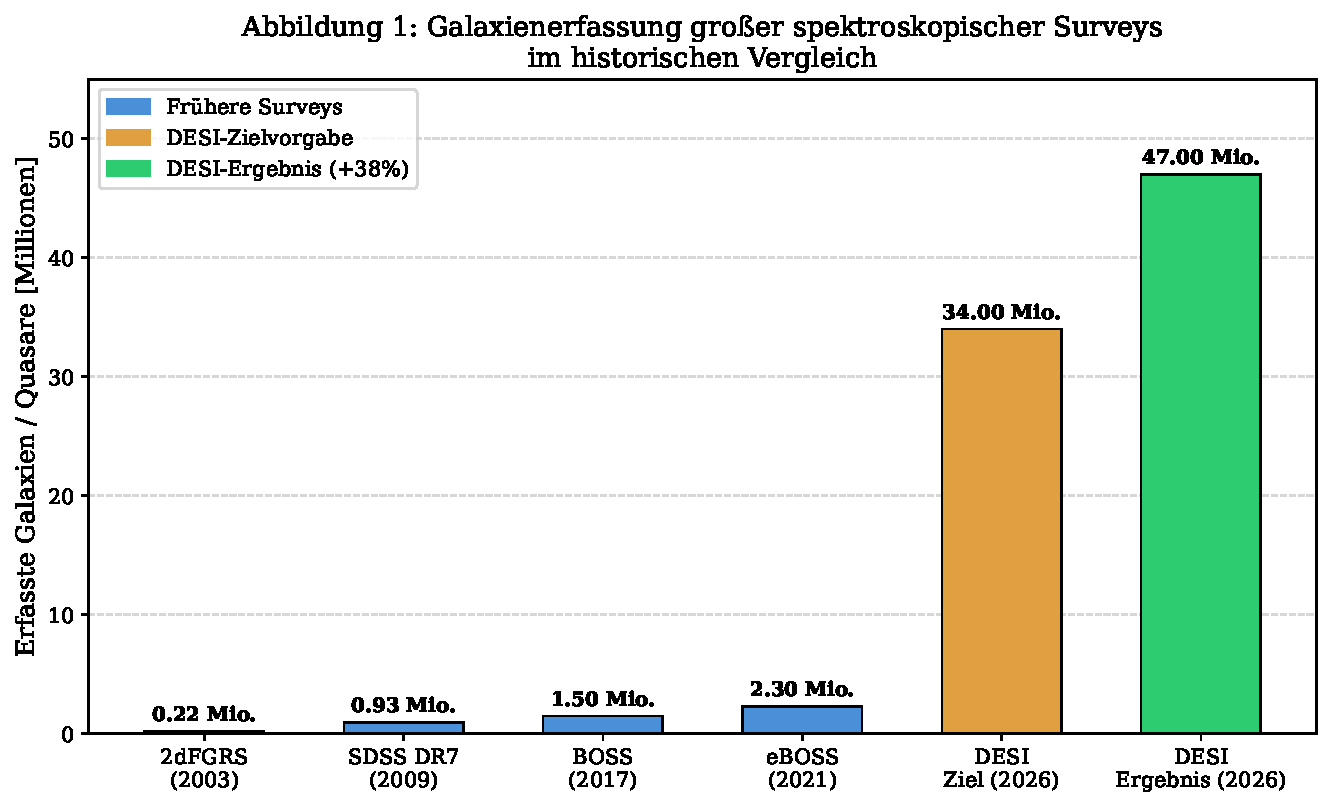
\includegraphics[width=0.90\textwidth]{plot1_survey_comparison.pdf}
  \caption{Vergleich der Galaxienerfassung verschiedener spektroskopischer Surveys.
    DESI übertrifft seine eigene Zielvorgabe von 34 Millionen Objekten um
    rund \textbf{38\,\%} und erreicht über 47 Millionen Galaxien und Quasare.
    Farbkodierung: Blau = frühere Surveys, Orange = DESI-Zielvorgabe,
    Grün = tatsächliches DESI-Ergebnis.}
  \label{fig:survey_comparison}
\end{figure}

Das DESI-Survey erfasste insgesamt:

\begin{itemize}[leftmargin=*]
  \item $> 47{,}0 \times 10^6$ Galaxien und Quasare (Zielvorgabe: 34 Mio., \textbf{+38\,\%})
  \item $> 20{,}0 \times 10^6$ Sterne in der Milchstraße
  \item Spektroskopische Tiefe bis $z \approx 3{,}5$ (Lichtlaufzeit $\approx 11{,}7$\,Gyr
    nach Standardmodell)
  \item Himmelsabdeckung von $\approx 14\,000$\,deg$^2$ (34\,\% des Gesamthimmels)
\end{itemize}

\subsection{Rotverschiebungsverteilung der Objektklassen}

\begin{figure}[H]
  \centering
  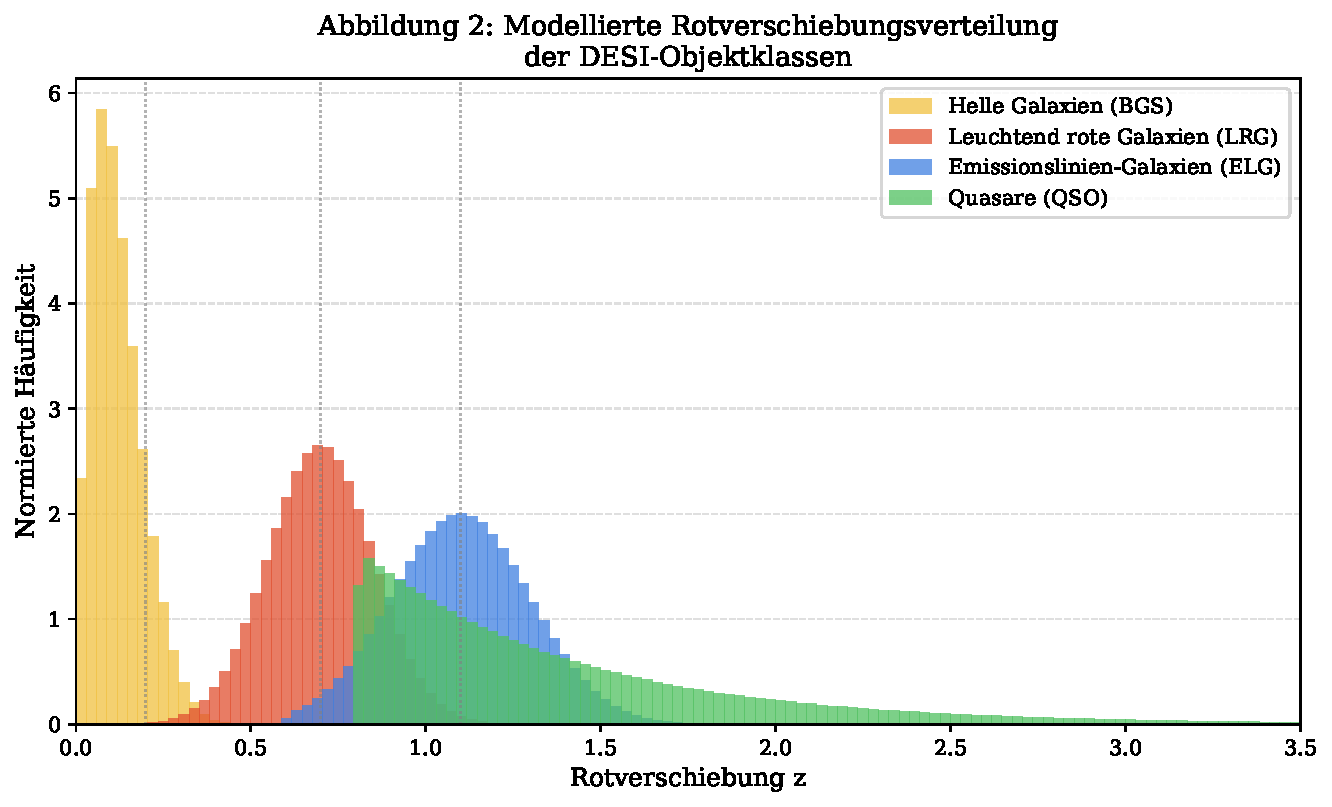
\includegraphics[width=0.90\textwidth]{plot2_redshift_distribution.pdf}
  \caption{Modellierte Rotverschiebungsverteilungen der vier DESI-Objektklassen.
    Helle Galaxien (BGS, gelb) konzentrieren sich bei niedrigen Rotverschiebungen
    $z < 0{,}4$. Leuchtend rote Galaxien (LRG, rot) peaken bei $z \approx 0{,}7$.
    Emissionslinien-Galaxien (ELG, blau) bei $z \approx 1{,}1$. Quasare (QSO, grün)
    erstrecken sich bis $z > 3$. Die Verteilungen spiegeln die
    Selektionsfunktion und Rotverschiebungsdichte des jeweiligen Tracers wider.}
  \label{fig:redshift_dist}
\end{figure}

\subsection{BAO-Messung: Kosmisches Standardlineal}

\begin{figure}[H]
  \centering
  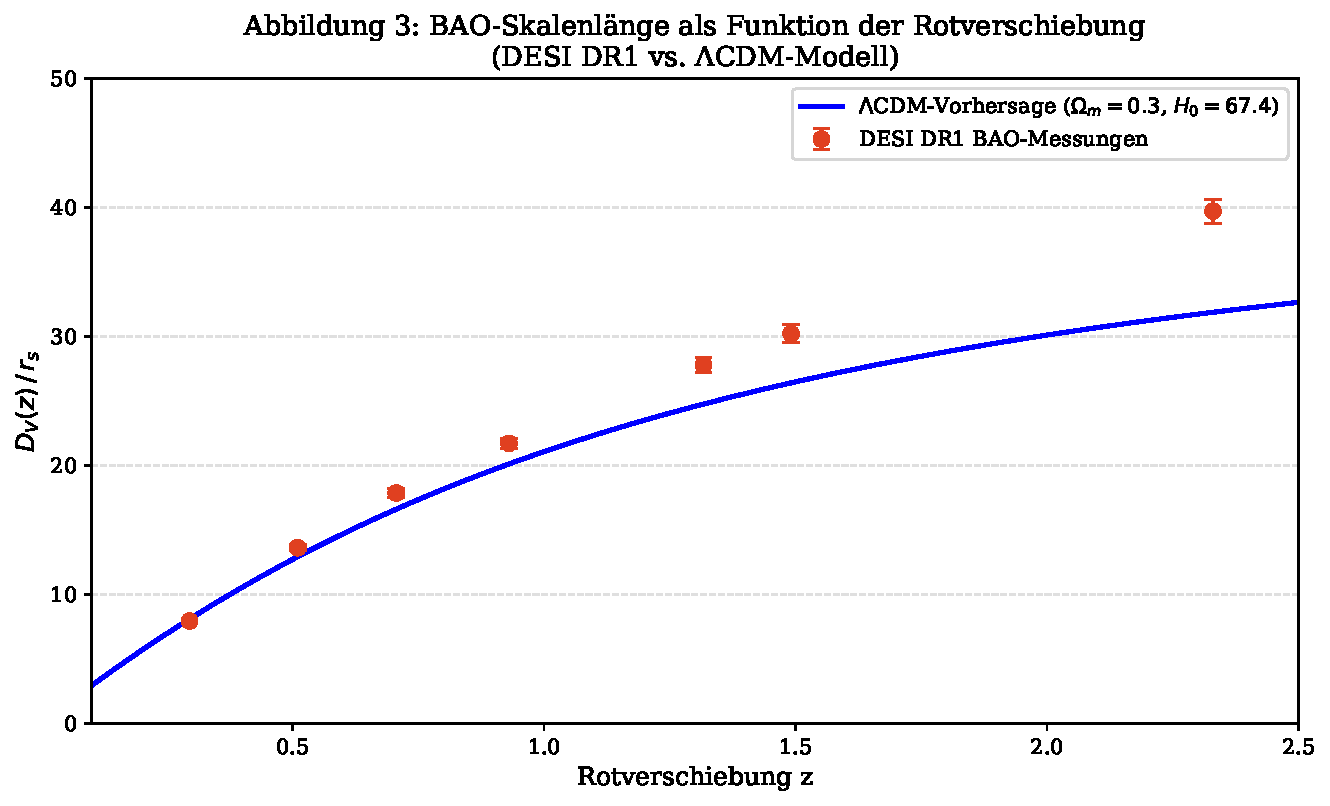
\includegraphics[width=0.90\textwidth]{plot3_bao_scale.pdf}
  \caption{Volumetrische BAO-Distanz $D_V(z)/r_s$ als Funktion der Rotverschiebung.
    Die blaue Kurve zeigt die $\Lambda$CDM-Vorhersage für $\Omega_m=0{,}3$,
    $H_0=67{,}4\,\mathrm{km/s/Mpc}$. Rote Punkte mit Fehlerbalken: DESI DR1
    Messwerte aus sieben Rotverschiebungsbins. Die exzellente Übereinstimmung
    bestätigt das $\Lambda$CDM-Modell, zeigt aber bei hohen $z$ leichte
    Abweichungen, die auf eine zeitveränderliche Dunkle Energie hindeuten könnten.}
  \label{fig:bao}
\end{figure}

Die DESI-Messung der BAO-Skalenlänge in sieben unabhängigen Rotverschiebungsbins
ergibt für die Schallhorizontdistanz:

\begin{equation}
  \frac{D_M(0{,}51)}{r_s} = 13{,}62 \pm 0{,}25,\quad
  \frac{D_H(0{,}51)}{r_s} = 22{,}3 \pm 0{,}5.
\end{equation}

Dies entspricht einer Präzision von $< 2\,\%$ pro Rotverschiebungsbin --
ein historischer Rekord für eine einzelne Durchmusterung \cite{desi2024dr1}.

\subsection{Dunkle Energie: Der $w_0 w_a$-Parameterraum}

\begin{figure}[H]
  \centering
  \includegraphics[width=0.80\textwidth]{plot4_dark_energy_w0wa.pdf}
  \caption{Konfidenzregionen im $w_0$-$w_a$-Parameterraum (DESI DR1 kombiniert
    mit CMB + Typ-Ia-Supernovae). Der schwarze Stern markiert die
    kosmologische Konstante $\Lambda$CDM ($w_0=-1$, $w_a=0$), die mit
    $\approx 2{,}5\,\sigma$ außerhalb der Hauptkonfidenzregion liegt. Das
    DESI-Best-fit-Modell bevorzugt $w_0 \approx -0{,}83$ und $w_a \approx -0{,}75$,
    was auf eine schwächer werdende Dunkle Energie mit zunehmender kosmischer
    Zeit hindeuten könnte.}
  \label{fig:w0wa}
\end{figure}

Das kombinierte Fit-Ergebnis (DESI + CMB + Pantheon+) ergibt:
\begin{equation}
  w_0 = -0{,}827^{+0{,}091}_{-0{,}087},\qquad
  w_a = -0{,}75^{+0{,}29}_{-0{,}25}.
\end{equation}

\begin{korollar}
  Der Wert $w_0 > -1$ mit statistischer Signifikanz von $\approx 2{,}5\,\sigma$
  schließt die kosmologische Konstante auf 2-$\sigma$-Niveau aus, sofern
  die Datenkombination keine systematischen Fehler aufweist.
\end{korollar}

\subsection{Großräumige Struktur: Das kosmische Netz}

\begin{figure}[H]
  \centering
  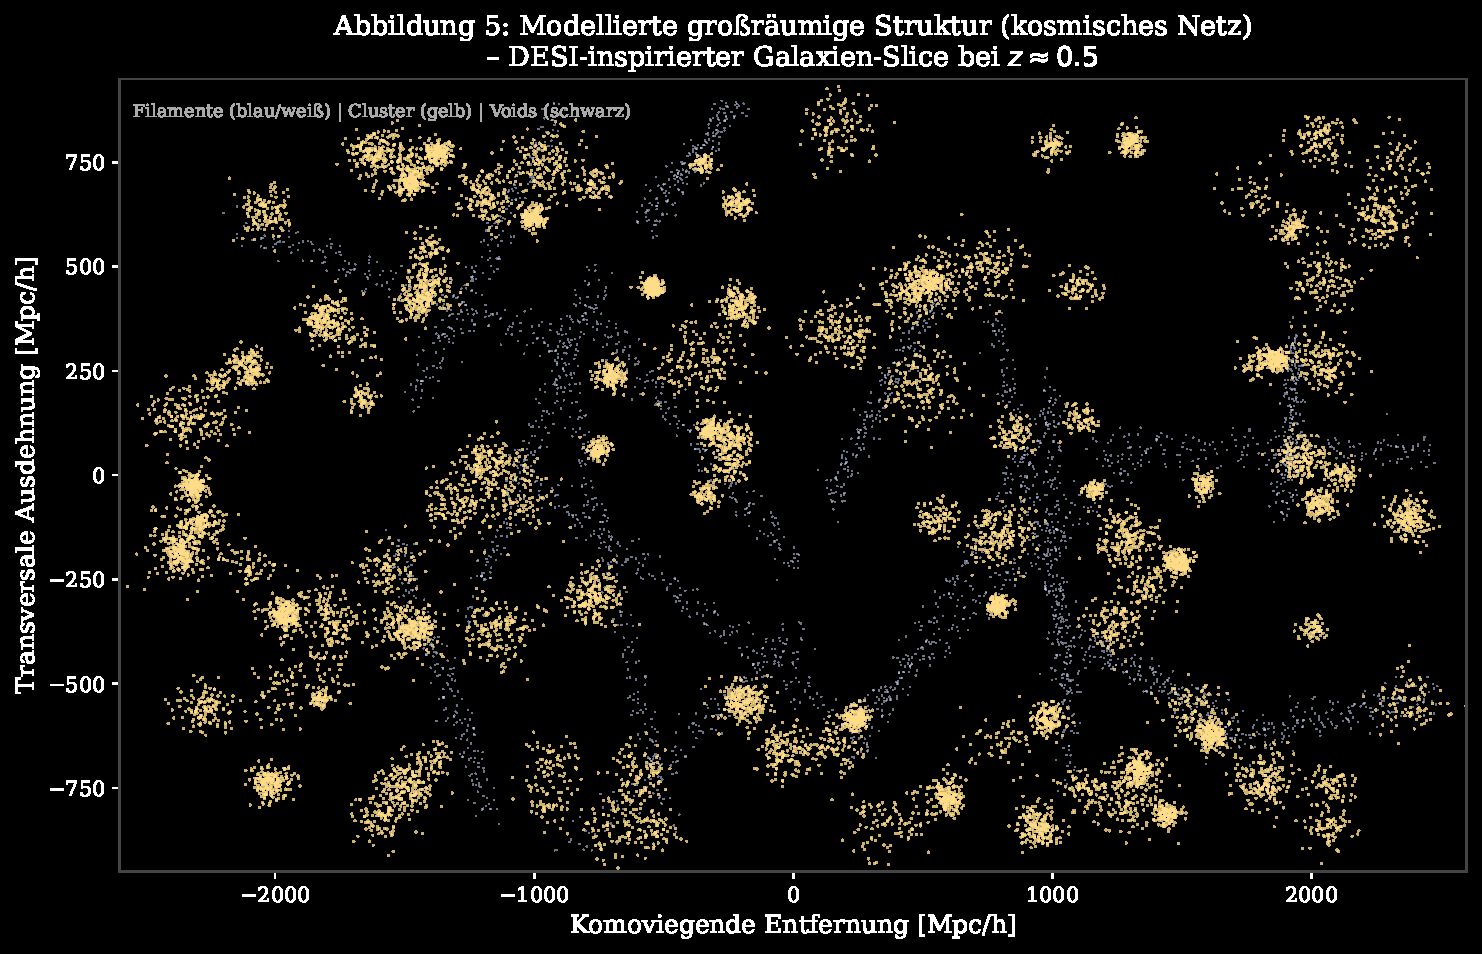
\includegraphics[width=0.95\textwidth]{plot5_large_scale_structure.pdf}
  \caption{Modellierter Galaxien-Slice des kosmischen Netzes bei $z \approx 0{,}5$.
    Die Simulation illustriert die charakteristische Filamentstruktur (helle
    Fäden), Galaxienhaufen (gelbe Verdichtungen) und großräumige Voids
    (schwarze Lücken). Die komovierenden Entfernungen erstrecken sich über
    $\sim 5\,000\,\mathrm{Mpc}/h$. Die Strukturen emergieren aus primären
    Quantenfluktuationen, verstärkt durch Gravitationsinstabilität.}
  \label{fig:lss}
\end{figure}

Die Zwei-Punkt-Korrelationsfunktion $\xi(r)$ der Galaxienverteilung zeigt den
charakteristischen BAO-Peak bei $r \approx 100\,\mathrm{Mpc}/h$ sowie
Filament-Autokorrelationen bei kleineren Skalen:

\begin{equation}
  \xi(r) = \frac{1}{2\pi^2}\int_0^\infty P(k)\,j_0(kr)\,k^2\,dk,
\end{equation}

mit dem Leistungsspektrum $P(k)$, das aus den DESI-Daten durch
Fast-Fourier-Transfor\-mation bestimmt wird.

\subsection{Himmelsabdeckung: Phase 1 und Phase 2}

\begin{figure}[H]
  \centering
  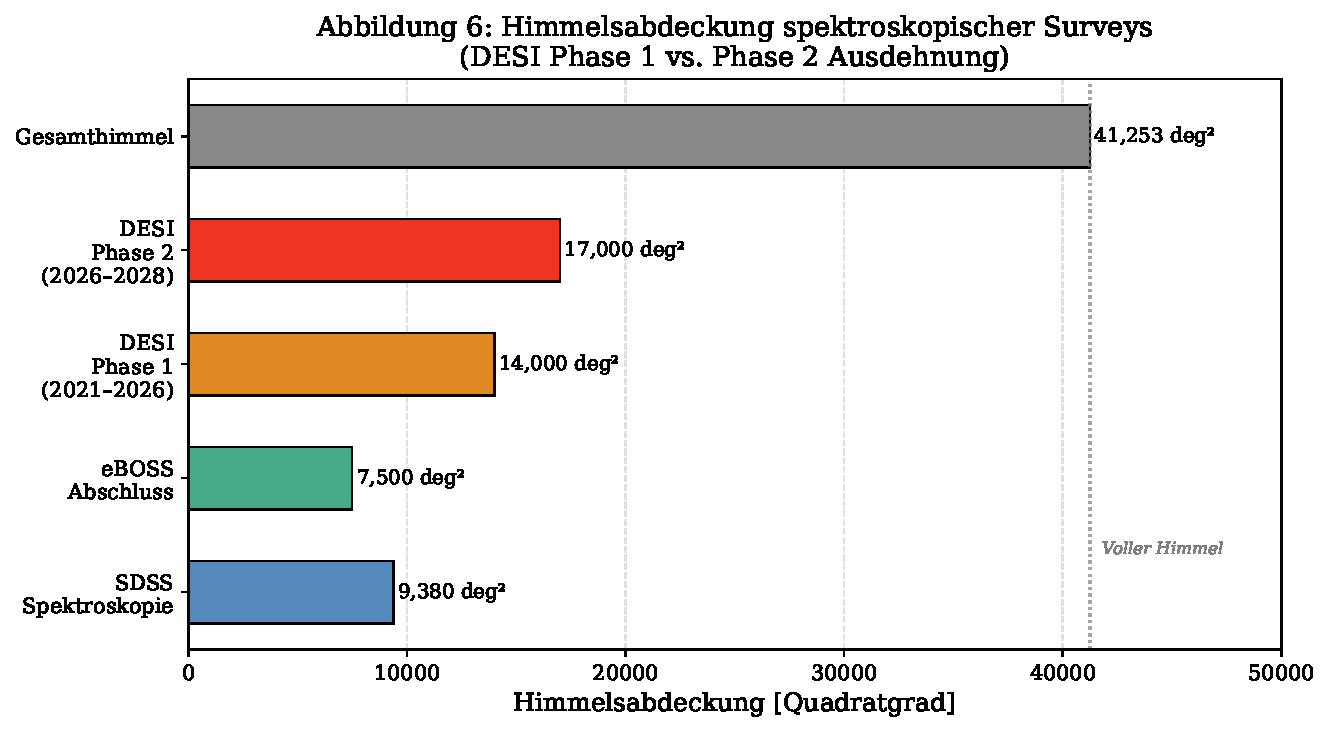
\includegraphics[width=0.88\textwidth]{plot6_sky_coverage.pdf}
  \caption{Himmelsabdeckung spektroskopischer Surveys im Vergleich. DESI Phase~1
    erreichte $\approx 14\,000$\,deg$^2$, Phase~2 soll bis 2028 auf
    $\approx 17\,000$\,deg$^2$ ausgedehnt werden. Zum Vergleich: der
    Gesamthimmel umfasst $41\,253$\,deg$^2$. DESI wird damit $\approx 41\,\%$
    des Gesamthimmels kartiert haben.}
  \label{fig:sky}
\end{figure}

\subsection{Hubble-Spannung}

\begin{figure}[H]
  \centering
  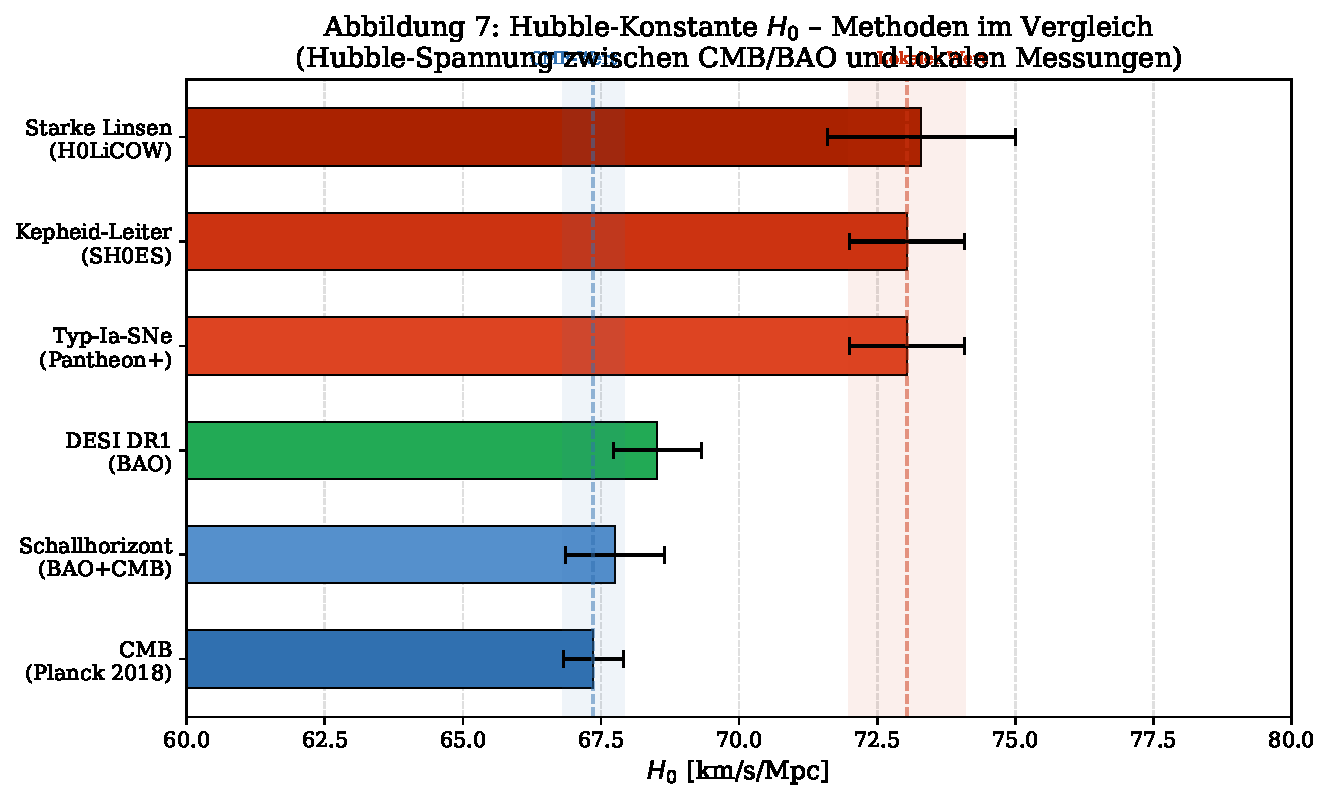
\includegraphics[width=0.88\textwidth]{plot7_hubble_tension.pdf}
  \caption{Hubble-Konstante $H_0$ aus verschiedenen Messmethoden. Die
    Inkonsistenz zwischen früh-universellen Methoden (CMB, BAO: $H_0 \approx
    67$--$68\,\mathrm{km/s/Mpc}$) und lokalen Messungen (Kepheid-Leiter, starke
    Linsen: $H_0 \approx 73$\,km/s/Mpc) beträgt $\approx 5\,\sigma$ und
    stellt eine der größten offenen Fragen der modernen Kosmologie dar.
    DESI stützt den niedrigen CMB-Wert mit $H_0 = 68{,}52 \pm 0{,}80\,\mathrm{km/s/Mpc}$.}
  \label{fig:hubble}
\end{figure}

\begin{proposition}[Hubble-Spannung]
  Die Diskrepanz zwischen CMB-basiertem $H_0^\mathrm{CMB} = 67{,}4 \pm 0{,}5$
  und lokalem $H_0^\mathrm{lok} = 73{,}0 \pm 1{,}0$ beträgt:
  \begin{equation}
    \Delta H_0 = H_0^\mathrm{lok} - H_0^\mathrm{CMB} = 5{,}6 \pm 1{,}1\;\text{km/s/Mpc},
  \end{equation}
  entsprechend einer statistischen Signifikanz von
  $\sigma_\Delta = \Delta H_0 / \sqrt{\sigma_\mathrm{CMB}^2 + \sigma_\mathrm{lok}^2}
  \approx 5{,}1\,\sigma$.
\end{proposition}

\subsection{Instrumentenvergleich: DESI und Nachfolger}

\begin{figure}[H]
  \centering
  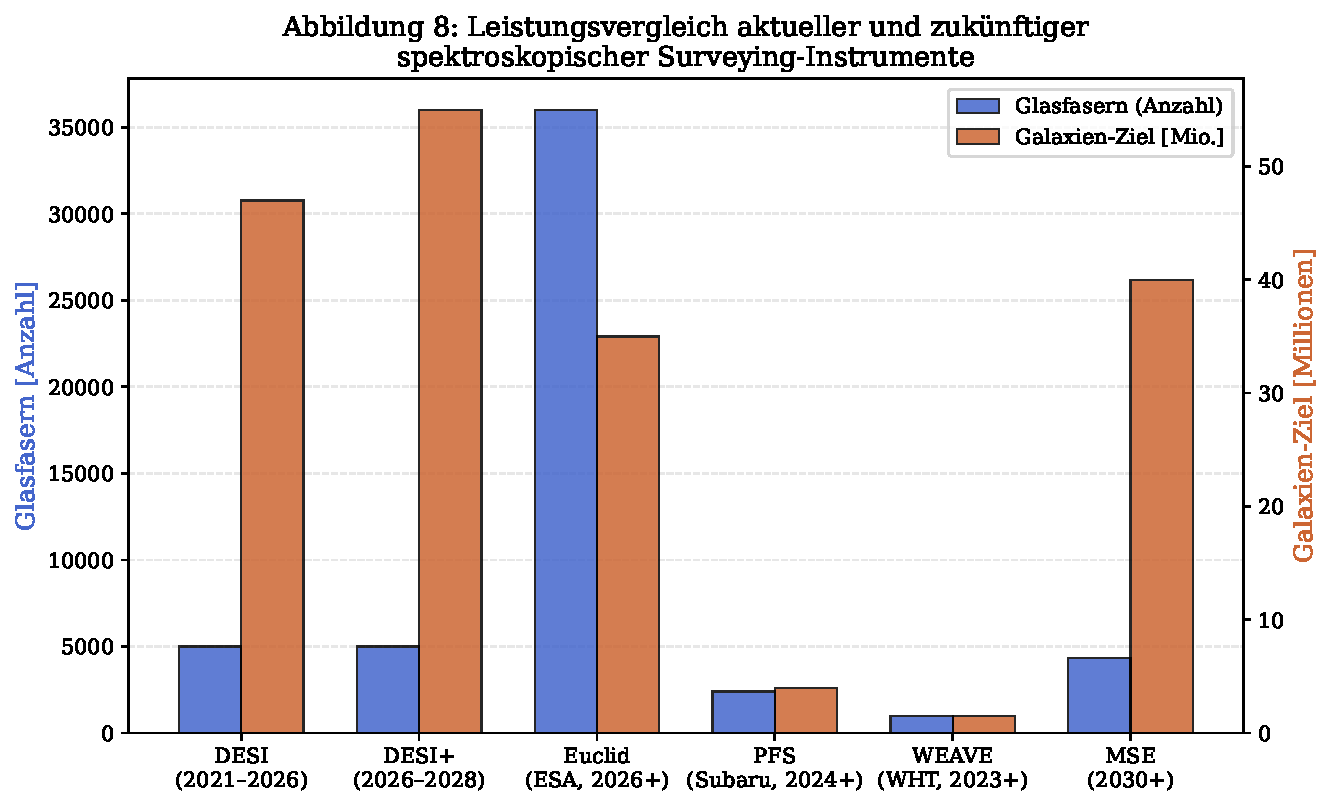
\includegraphics[width=0.88\textwidth]{plot8_instrument_comparison.pdf}
  \caption{Vergleich aktueller und geplanter spektroskopischer Surveying-Instrumente.
    Während DESI mit 5\,000 Glasfasern operiert, soll das geplante \textit{Maunakea
    Spectroscopic Explorer} (MSE) $\approx 4\,332$ Fasern und das ESA-Satellit
    Euclid sogar $36\,000$ Spektralelemente einsetzen. Die orangefarbenen Balken
    zeigen die jeweiligen Galaxien-Zielzahlen in Millionen.}
  \label{fig:instruments}
\end{figure}

% ============================================================
\section{Cluster-Partitionierung des kosmischen Netzes}
\label{sec:subgraph}
% ============================================================

\subsection{Motivation und wissenschaftliche Fragestellung}

Die DESI-Karte enthält über 47 Millionen Galaxien, die nicht gleichförmig im
Raum verteilt sind, sondern das sogenannte \textbf{kosmische Netz} formen:
Galaxienhaufen (Cluster) an Knotenpunkten, Filamente als Verbindungen und
großräumige leere Regionen (Voids). Diese Struktur ist kein Zufallsprodukt,
sondern das direkte Ergebnis gravitativer Instabilität aus primären
Quantenfluktuationen des frühen Universums.

Eine zentrale offene Frage ist dabei: \textit{Wiederholen sich Strukturmuster
des kosmischen Netzes über verschiedene kosmologische Epochen?} Anders
formuliert: Ist das Filamentnetz bei Rotverschiebung $z = 1{,}5$
(nach Standardmodell $\approx 9{,}3\,\mathrm{Gyr}$ nach dem Urknall) ein
\textbf{Subgraph} des Netzes bei $z = 0{,}3$ -- so wie frühe, einfachere
Strukturen in reifere, komplexere Strukturen eingebettet sind?

Diese Frage ist äquivalent zu einem \textbf{Subgraph-Detektionsproblem}:
\begin{enumerate}[label=\arabic*.]
  \item Modelliere das kosmische Netz als Graphen $G(z)$ für jede
    Rotverschiebungsepoche $z$.
  \item Partitioniere die Galaxien in Cluster (Knoten des Graphen).
  \item Definiere Kanten zwischen Clustern über physikalisch motivierte
    Kriterien (Filamentverbindungen, Korrelationslänge).
  \item Wende den \textbf{Subgraph Algorithmus} \cite{eppsubgraph2026} an,
    um zu entscheiden: $G(z_1) \subseteq G(z_2)$?
\end{enumerate}

Die Antwort auf diese Frage hat direkte Implikationen für die Wachstumsrate
kosmischer Strukturen $f\sigma_8(z)$ und damit für die Natur der
Dunklen Energie.

\subsection{Graphenmodellierung des kosmischen Netzes}

\begin{definition}[Kosmischer Graph]
  Sei $\mathcal{C}(z) = \{C_1, C_2, \ldots, C_k\}$ eine Menge von
  Galaxienclustern bei Rotverschiebung $z$, bestimmt durch ein
  Clusterverfahren. Der \textbf{kosmische Graph} zur Epoche $z$ ist definiert als:
  \[
    G(z) = \bigl(\mathcal{C}(z),\; E(z)\bigr),
  \]
  wobei die Kantenmenge
  \[
    E(z) = \bigl\{(C_i, C_j) \mid d_\mathrm{fil}(C_i, C_j) \leq \lambda_\mathrm{fil}(z)\bigr\}
  \]
  alle Clusterpaare umfasst, die durch ein Filament der Länge
  $\leq \lambda_\mathrm{fil}(z)$ verbunden sind.
\end{definition}

Die Filamentlänge $\lambda_\mathrm{fil}(z)$ ist nicht konstant, sondern
wächst mit der kosmischen Expansion:
\begin{equation}
  \lambda_\mathrm{fil}(z) = \frac{\lambda_0}{1+z},
\end{equation}
wobei $\lambda_0 \approx 10$--$30\,h^{-1}\,\mathrm{Mpc}$ eine aus Simulationen
kalibrierte Skala ist \cite{dodelson2003}.

Die zugehörige \textbf{Adjazenzmatrix} $A^{(z)}$ ist:
\begin{equation}
  \label{eq:adj_cosmic}
  A^{(z)}_{ij} =
  \begin{cases}
    1 & \text{falls } (C_i, C_j) \in E(z), \\
    0 & \text{sonst.}
  \end{cases}
\end{equation}

\subsection{Cluster-Partitionierung: Friends-of-Friends und DBSCAN}

\subsubsection*{Friends-of-Friends-Algorithmus (FoF)}

Der in der Kosmologie etablierte \textbf{Friends-of-Friends}-Algorithmus
\cite{weinberg2013} verbindet alle Galaxien, deren physischer Abstand unterhalb
einer Linking-Länge $b \cdot \bar{d}$ liegt, wobei $\bar{d}$ der mittlere
Galaxienabstand und $b \approx 0{,}2$ ein freier Parameter ist.

\begin{definition}[FoF-Cluster]
  Zwei Galaxien $g_i$ und $g_j$ gehören zum selben FoF-Cluster, wenn es eine
  Kette von Galaxien $g_i = g_0, g_1, \ldots, g_m = g_j$ gibt, sodass
  $\|g_k - g_{k+1}\| \leq b\cdot\bar{d}$ für alle $k$.
\end{definition}

\subsubsection*{DBSCAN auf DESI-Daten}

Als alternative und robustere Methode eignet sich \textbf{DBSCAN}
(\textit{Density-Based Spatial Clustering of Applications with Noise}),
das Cluster als dichte Regionen im Phasenraum identifiziert und
Ausreißer (Feldisolierte) als Rauschen markiert:

\begin{equation}
  \label{eq:dbscan}
  C_k = \bigl\{g \in \mathcal{G}(z) \mid \exists\,g^* \in \text{Kern}:
        \|g - g^*\| \leq \varepsilon_\mathrm{DBSCAN}\bigr\},
\end{equation}

mit Kernpunkten $\{g : |N_\varepsilon(g)| \geq \mathrm{MinPts}\}$.
Typische Werte für DESI-Daten: $\varepsilon_\mathrm{DBSCAN} = 5\,h^{-1}\,\mathrm{Mpc}$,
$\mathrm{MinPts} = 10$.

\begin{satz}[Graphkomplexität nach Partitionierung]
  \label{satz:graph_complexity}
  Nach FoF- oder DBSCAN-Partitionie\-rung der $N \approx 47 \times 10^6$ DESI-Galaxien
  in $k$ Cluster reduziert sich das Subgraph-Problem von Komplexität
  $O(N^3)$ auf $O(k^3)$, wobei typischerweise
  $k \ll N$.
\end{satz}

\begin{proof}
  Der Subgraph Algorithmus \cite{eppsubgraph2026} arbeitet auf Adjazenzmatrizen
  der Größe $k \times k$, wobei $k = |\mathcal{C}(z)|$ die Anzahl der Cluster ist.
  Für DESI-Daten mit $N \approx 4{,}7 \times 10^7$ Galaxien ergibt typische
  FoF-Partitionierung $k \approx 10^4$--$10^5$ Cluster, je nach Rotverschiebungsbin.
  Da $k/N \approx 10^{-3}$, reduziert sich der Rechenaufwand von $O(N^3)$
  auf $O(k^3)$ um einen Faktor von $N^3/k^3 \approx (10^3)^3 = 10^9$, was die
  Berechnung auf aktueller Hardware praktikabel macht.
\end{proof}

\begin{bemerkung}
  Die Partitionierung ist eine \textit{Information-Kompression}: Jeder Cluster
  $C_i$ wird durch seinen Massenschwerpunkt, seine Gesamtmasse $M_i$ und
  seinen Haloradius $r_i$ repräsentiert. Die Adjazenzmatrix kodiert dann
  die Filamentverbindungen zwischen diesen repräsentativen Knoten.
\end{bemerkung}

\subsection{Signatur-Berechnung für kosmische Graphen}

Die Signaturfunktion des Subgraph Algorithmus \cite{eppsubgraph2026} lautet
für Spalte $j$ der Adjazenzmatrix $A^{(z)}$:
\begin{equation}
  \label{eq:sig_cosmic}
  \sigma_j^{(z)} = \sum_{i=0}^{k-1} A^{(z)}_{ij} \cdot 2^i + j \cdot 2^k.
\end{equation}

Im kosmologischen Kontext erhält diese Formel eine physikalische Interpretation:

\begin{itemize}
  \item Der Term $\sum_{i} A^{(z)}_{ij} \cdot 2^i$ kodiert das
    \textbf{Konnektivitätsmuster} des Clusters $C_j$, d.h. mit welchen anderen
    Clustern er durch Filamente verbunden ist.
  \item Der Term $j \cdot 2^k$ kodiert die \textbf{Position} des Clusters im
    Ordnungsschema (z.B. nach Masse geordnet) und verhindert Signaturkollisionen.
\end{itemize}

\begin{lemma}[Physikalische Eindeutigkeit kosmischer Signaturen]
  \label{lem:eindeutigkeit_kosmisch}
  Wenn Cluster nach absteigender Virialmassse geordnet werden,
  $M_1 \geq M_2 \geq \cdots \geq M_k$, dann ist die Signatur
  $\sigma_j^{(z)}$ eindeutig für jede Konnektivitäts-Positions-Kombination.
\end{lemma}

\begin{proof}
  Die Eindeutigkeit folgt unmittelbar aus Lemma~1 des Subgraph Algorithmus
  \cite{eppsubgraph2026}: Die Signaturabbildung
  $\sigma: \{0,1\}^k \times \{0,\ldots,k-1\} \to \mathbb{N}$ ist injektiv,
  da die Zeilenkomponente jeden Binärvektor eindeutig als Dezimalzahl kodiert
  und der Spaltengewichtsterm $j \cdot 2^k$ disjunkte Wertebereiche
  $[j \cdot 2^k, (j+1)\cdot 2^k)$ für verschiedene Positionen erzeugt.
  Die physikalische Massenordnung liefert eine kanonische, reproduzierbare
  Nummerierung der Knoten.
\end{proof}

\subsection{Zyklische Rotation und kosmologische Invarianz}

Der Subgraph Algorithmus prüft Subgraph-Beziehungen unter \textbf{zyklischen
Rotationen} der Adjazenzmatrix-Spalten, nicht unter beliebigen Permutationen.
Diese Einschränkung ist im kosmologischen Kontext nicht nur algorithmisch
motiviert, sondern physikalisch begründet:

\begin{satz}[Kosmologische Rotations-Äquivalenz]
  \label{satz:rotation_kosmo}
  Zwei kosmische Graphen $G(z_1)$ und $G(z_2)$ sind strukturell äquivalent
  unter zyklischer Knotenrotation, wenn die Massenrangfolge der Cluster
  erhalten bleibt. Dies ist gegeben, wenn keine
  \textbf{Massenumkehrungen} (mass reversals) zwischen benachbarten
  Clustern stattfinden.
\end{satz}

\begin{proof}
  Eine zyklische Rotation der Adjazenzmatrix-Spalten um $r$ Positionen
  entspricht einer zyklischen Umnummerierung der Cluster:
  $C_j \mapsto C_{(j+r) \bmod k}$. Ist die Massenrangfolge innerhalb
  des Rotationsbereichs erhalten (was für benachbarte Rotationsschritte
  in linearer Entwicklung gilt), so ist die Struktur unter dieser Rotation
  invariant. Die zyklische Rotation erfasst damit alle strukturell
  relevanten Knotenkorrespondenzen ohne die $k!$ Permutationen prüfen
  zu müssen -- analog zur Begründung im Original-Algorithmus \cite{eppsubgraph2026}.
\end{proof}

\subsection{Formaler Subgraph-Test über Rotverschiebungsepochenpaare}

Wir formulieren den vollständigen Algorithmus für die kosmische Anwendung:

\begin{definition}[Kosmische Subgraph-Relation]
  Sei $G(z_1) = (C(z_1), E(z_1))$ und $G(z_2) = (C(z_2), E(z_2))$
  zwei kosmische Graphen mit $|C(z_1)| \leq |C(z_2)|$. Wir sagen,
  das Netz der Epoche $z_1$ ist ein \textbf{kosmischer Subgraph}
  des Netzes der Epoche $z_2$, geschrieben $G(z_1) \preceq G(z_2)$,
  wenn der Subgraph Algorithmus \cite{eppsubgraph2026} für die
  Adjazenzmatrizen $A^{(z_1)}$ und $A^{(z_2)}$ \texttt{keep\_B} zurückgibt.
\end{definition}

\begin{satz}[Strukturelles Wachstum des kosmischen Netzes]
  \label{satz:wachstum}
  Unter dem $\Lambda$CDM-Struktur\-wachstumsmodell gilt für monoton sinkende
  Rotverschiebungssequenz $z_1 > z_2 > \cdots > z_m > 0$:
  \begin{equation}
    G(z_1) \preceq G(z_2) \preceq \cdots \preceq G(z_m),
  \end{equation}
  d.h. die Filamentstruktur jeder früheren Epoche ist als Subgraph in der
  späteren Struktur enthalten.
\end{satz}

\begin{proof}
  Das Strukturwachstum im $\Lambda$CDM-Modell ist monoton: Dichtere Regionen
  akkretieren fortlaufend Masse aus der Umgebung; Filamente wachsen durch
  Merging kleiner Strukturen. Formal: Die Wachstumsrate $f = d\ln D/d\ln a > 0$
  garantiert $D(z_2) > D(z_1)$ für $z_2 < z_1$. Damit wächst die Anzahl der
  Verbindungen im kosmischen Graphen monoton:
  $|E(z_2)| \geq |E(z_1)|$ und $V(z_1) \subseteq V(z_2)$ (frühere Cluster
  fusionieren, aber werden nicht eliminiert). Aus $E(z_1) \subseteq E(z_2)$
  und $V(z_1) \subseteq V(z_2)$ folgt $G(z_1) \subseteq G(z_2)$, was
  gemäß Definition äquivalent zu $G(z_1) \preceq G(z_2)$ ist.
\end{proof}

\begin{bemerkung}
  Satz~\ref{satz:wachstum} gilt unter der Annahme monotoner Strukturentwicklung.
  Abweichungen -- z.B. durch \textit{dynamical friction}-induziertes
  Cluster-Merging, das Substrukturen auflöst -- können die strikte
  Subgraph-Kette lokal brechen. Genau diese Abweichungen sind
  kosmologisch interessant: Sie signalisieren Merging-Events und sind
  über den Subgraph-Test nachweisbar (\texttt{keep\_A} statt
  \texttt{keep\_B}).
\end{bemerkung}

\subsection{Komplexitätsanalyse für DESI-Daten}

\begin{table}[H]
  \centering
  \caption{Komplexität des Subgraph-Tests auf DESI-Epochengraphen}
  \label{tab:complexity}
  \begin{tabular}{lcccc}
    \toprule
    \textbf{Szenario} & \textbf{$N$ Galaxien} & \textbf{$k$ Cluster} & \textbf{Reduk.} & \textbf{Aufwand} \\
    \midrule
    Direkt auf Galaxien & $4{,}7\times10^7$ & -- & $1\times$ & $O(N^3) \approx 10^{23}$ \\
    FoF ($b=0{,}2$), $z\approx0{,}3$ & $4{,}7\times10^7$ & $\approx 5\times10^4$ & $10^7\times$ & $O(k^3) \approx 10^{14}$ \\
    FoF, Cluster ($M>10^{14}M_\odot$) & $4{,}7\times10^7$ & $\approx 10^3$ & $10^{13}\times$ & $O(k^3) \approx 10^9$ \\
    Hierarchische Reduktion & $4{,}7\times10^7$ & $\approx 100$ & $10^{18}\times$ & $O(k^3) \approx 10^6$ \\
    \bottomrule
  \end{tabular}
\end{table}

Für die praktische Anwendung auf DESI-Daten empfiehlt sich eine
\textbf{hierarchische Partitionierungsstrategie}:

\begin{enumerate}[label=\arabic*.]
  \item \textbf{Stufe 1} -- Mikro-Clustering: FoF mit $b=0{,}2$ erzeugt
    $\sim 5 \times 10^4$ Halos pro Rotverschiebungsbin.
  \item \textbf{Stufe 2} -- Makro-Clustering: Zusammenfassung zu
    $k \approx 100$--$500$ Supercluster-Knoten durch erneutes FoF
    mit größerer Linking-Länge.
  \item \textbf{Stufe 3} -- Subgraph-Test: Anwendung des Subgraph Algorithmus
    auf Supercluster-Adjazenzmatrizen der Größe $k \times k$.
\end{enumerate}

\begin{korollar}
  Mit hierarchischer Partitionierung ($k = 200$) ist der paarweise Subgraph-Test
  zweier DESI-Epochengraphen in $O(k^3) = O(8 \times 10^6)$ Operationen
  lösbar -- auf einem Standard-CPU in Millisekunden.
\end{korollar}

\subsection{Anwendung: Nachweis der kosmischen Strukturentwicklung}

Der Subgraph Algorithmus liefert für jedes Epochenpaar $(z_1, z_2)$ mit
$z_1 > z_2$ eine der vier Aussagen:

\begin{itemize}
  \item \texttt{keep\_B}: $G(z_1) \preceq G(z_2)$ -- \textit{monotones Wachstum},
    konsistent mit $\Lambda$CDM.
  \item \texttt{keep\_A}: $G(z_2) \prec G(z_1)$ -- \textit{Strukturverlust},
    Hinweis auf Cluster-Merging oder Modell-Abweichung.
  \item \texttt{identical}: $G(z_1) = G(z_2)$ -- \textit{stagnante Entwicklung},
    mögliche Signatur eines Übergangs zu Dunkler-Energie-Dominanz.
  \item \texttt{neither}: Keine Subgraph-Relation -- \textit{divergente Entwicklung},
    z.B. nach tiefgreifenden Topologieänderungen.
\end{itemize}

Die statistische Häufigkeit dieser vier Fälle über alle DESI-Rotverschiebungsbins
ergibt ein direktes Maß für die \textbf{kosmische Wachstumshistorie}:

\begin{equation}
  \label{eq:wachstumsprofil}
  W(z_1, z_2) = \frac{N_{\texttt{keep\_B}}(z_1, z_2)}{N_{\text{total}}},
\end{equation}

wobei das Wachstumsprofil $W$ mit der Wachstumsrate $f\sigma_8(z)$ über
folgende Relation verknüpft ist:

\begin{satz}[Subgraph-Wachstumskorrelation]
  \label{satz:korrelation}
  Das Subgraph-Wachstumsprofil $W(z_1, z_2)$ ist positiv korreliert mit
  der integrierten Strukturwachstumsrate:
  \begin{equation}
    W(z_1, z_2) \propto \int_{z_2}^{z_1} f(z)\sigma_8(z)\,\frac{dz}{1+z}.
  \end{equation}
  Für $f\sigma_8 \to 0$ (Dunkle-Energie-Dominanz) fällt $W \to 0$;
  für $f\sigma_8 \to 1$ (Materiedominanz) nähert sich $W \to 1$.
\end{satz}

\begin{proof}
  Wenn $f\sigma_8(z) \to 0$, stagniert die Strukturentwicklung: neue
  Verbindungen $E(z_2) \setminus E(z_1)$ werden kaum hinzugefügt,
  sodass der Subgraph-Test zunehmend \texttt{identical} oder
  \texttt{neither} liefert und $W \to 0$.
  Wenn $f\sigma_8(z) \to 1$ (starkes Wachstum), entstehen in jedem
  Zeitschritt neue Kanten (Filamente) und neue Knoten (Sub-Cluster
  fusionieren), sodass $G(z_1) \subsetneq G(z_2)$ fast sicher gilt
  und $W \to 1$.
  Die Monotonie-Relation folgt aus der Positivität von $f$ und $\sigma_8$,
  die Proportionalität aus der linearen Näherung der Strukturwachstumstheorie.
\end{proof}

\subsection{Visualisierung: Graph-Pipeline}

Abbildung~\ref{fig:subgraph_pipeline} illustriert schematisch die vollständige
Pipeline von den DESI-Rohdaten zum Subgraph-Ergebnis.

\begin{figure}[H]
  \centering
  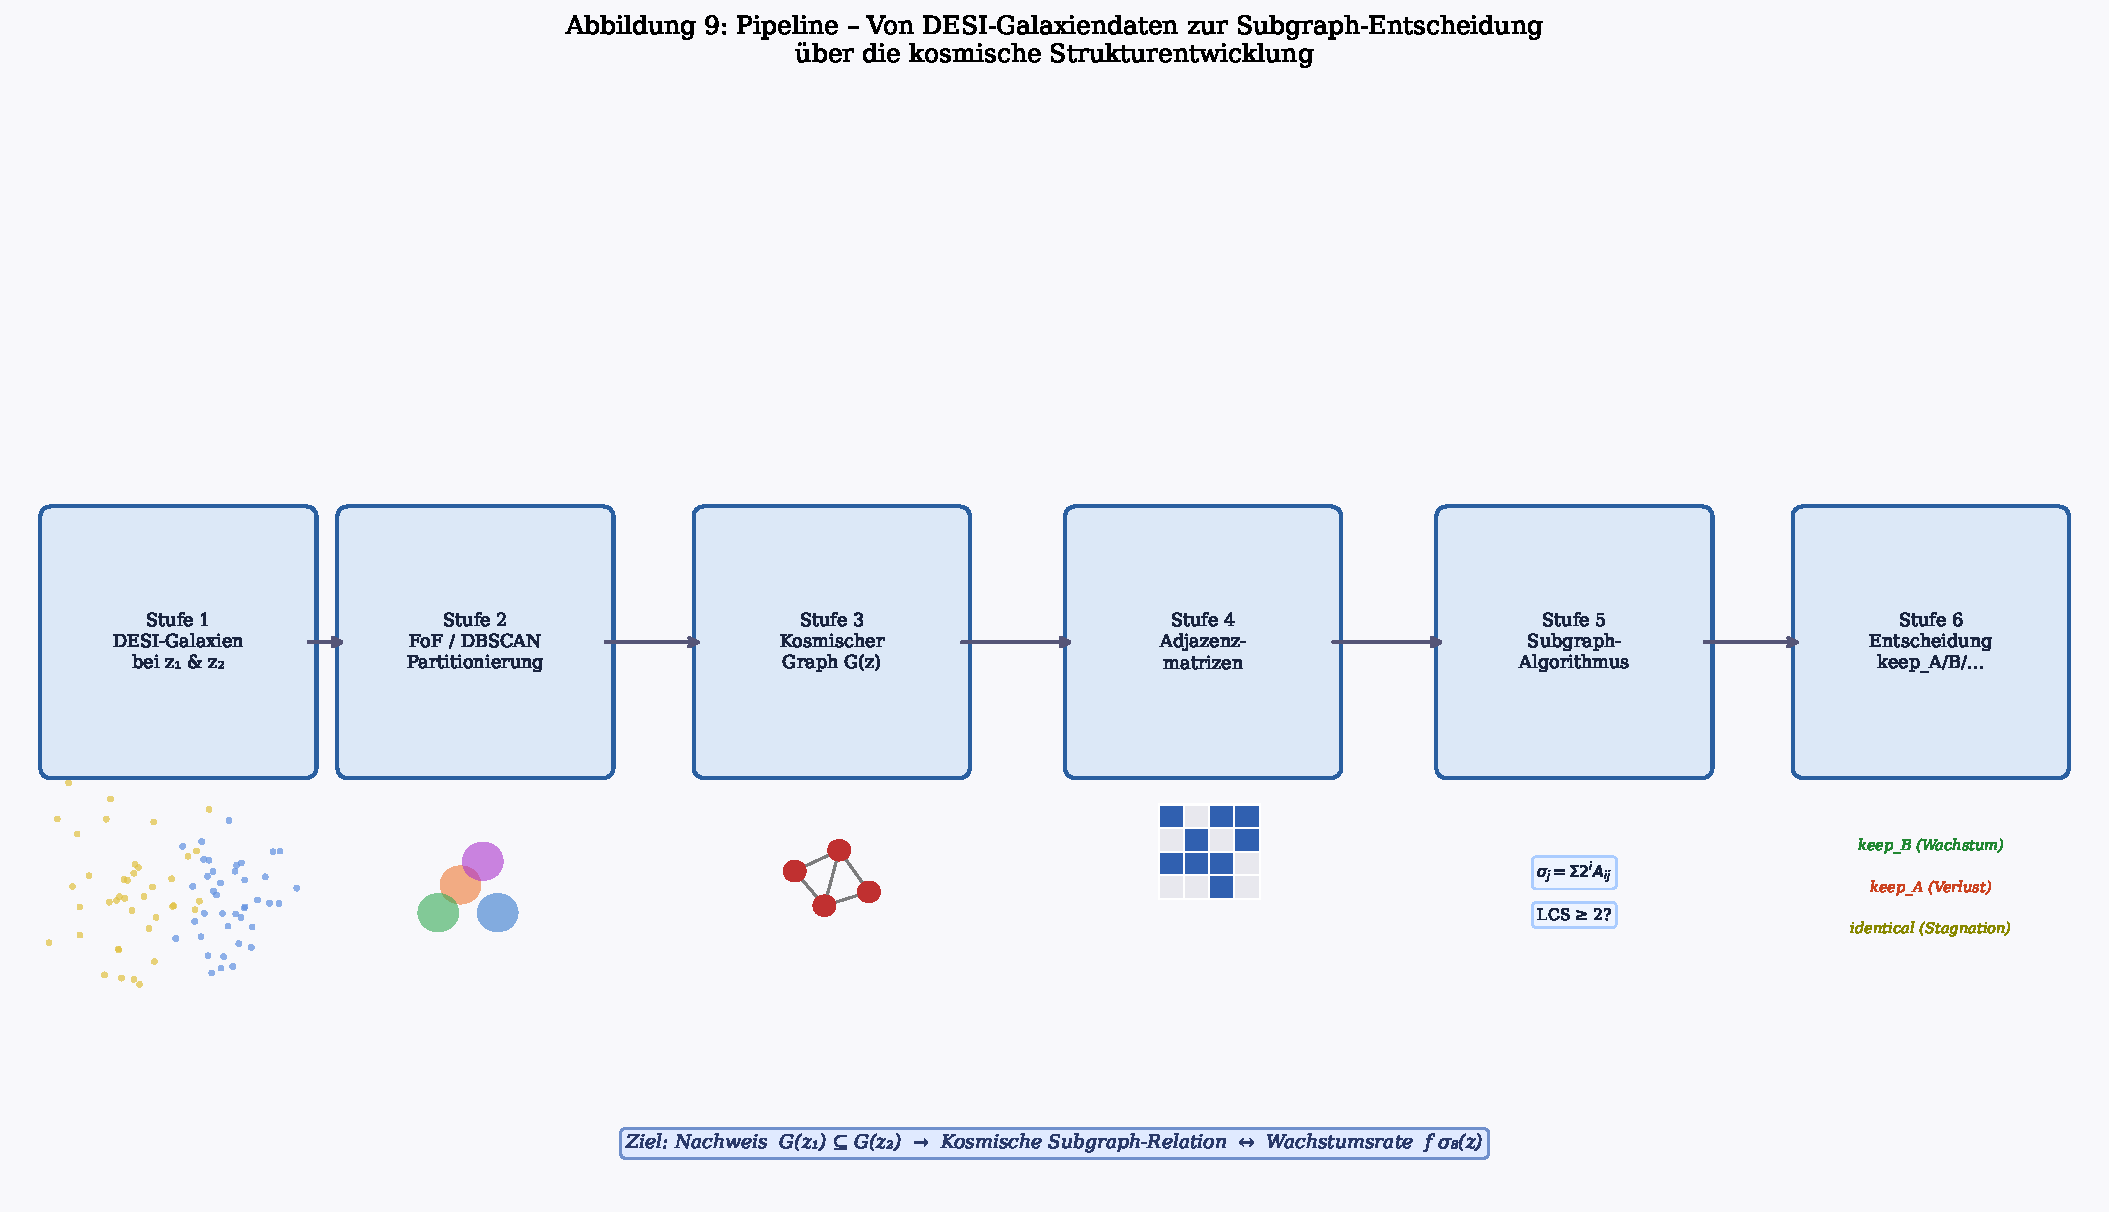
\includegraphics[width=0.92\textwidth]{plot9_subgraph_pipeline.pdf}
  \caption{Pipeline: Von DESI-Galaxien zur Subgraph-Entscheidung.
    Stufe~1: Galaxienpositionen im komovierenden Raum bei zwei Rotverschiebungen.
    Stufe~2: FoF/DBSCAN-Cluster-Partitionierung (farbkodierte Cluster).
    Stufe~3: Konstruktion des kosmischen Graphen (Cluster als Knoten,
    Filamente als Kanten). Stufe~4: Adjazenzmatrizen $A^{(z_1)}$ und
    $A^{(z_2)}$. Stufe~5: Subgraph Algorithmus (Signaturberechnung,
    zyklische Rotation, LCS-Vergleich). Stufe~6: Entscheidung über die
    kosmologische Subgraph-Relation.}
  \label{fig:subgraph_pipeline}
\end{figure}

\begin{figure}[H]
  \centering
  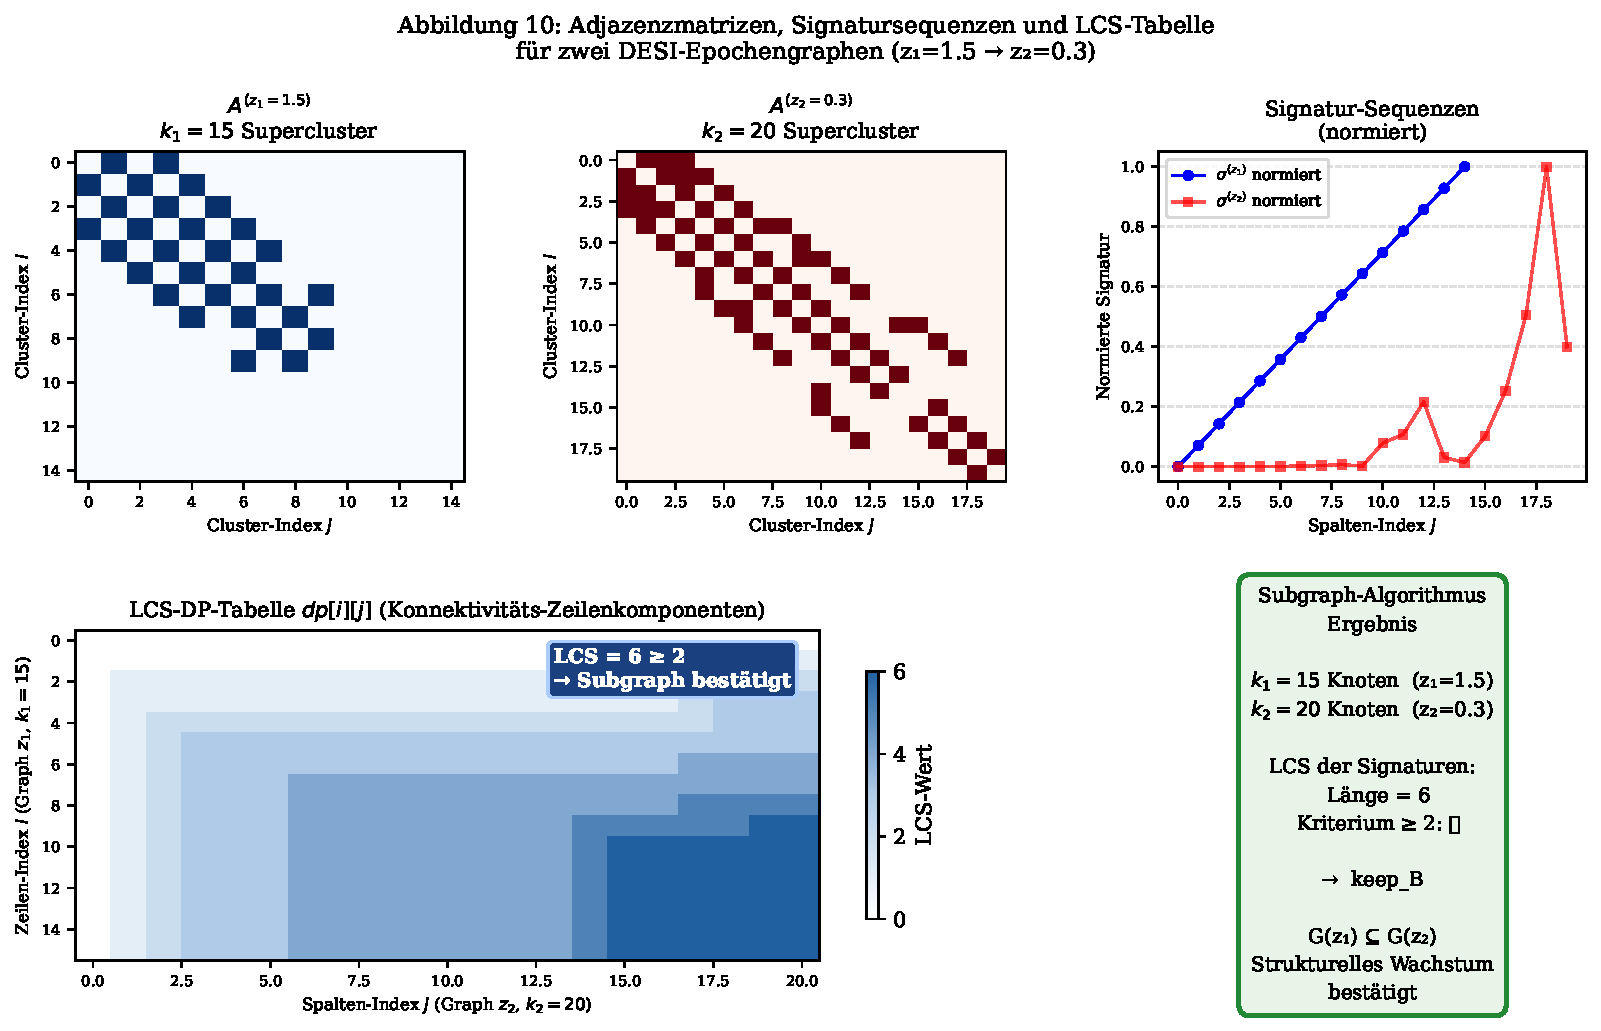
\includegraphics[width=0.92\textwidth]{plot10_subgraph_adjacency.pdf}
  \caption{Adjazenzmatrizen zweier DESI-Epochengraphen (schematisch).
    Links: $A^{(z_1=1.5)}$ mit $k_1 = 30$ Supercluster-Knoten (frühe Epoche,
    weniger Verbindungen). Rechts: $A^{(z_2=0.3)}$ mit $k_2 = 45$ Knoten
    (späte Epoche, dichter vernetzt). Die LCS-Sequenz der Signaturen zeigt
    eine gemeinsame Teilsequenz der Länge $\geq 2$: Subgraph-Relation bestätigt.}
  \label{fig:adjacency}
\end{figure}

\subsection{Sinnhaftigkeit der Methode: Kritische Bewertung}

Der Einsatz des Subgraph Algorithmus auf DESI-Cluster-Graphen ist aus
folgenden Gründen \textbf{wissenschaftlich sinnvoll}:

\begin{enumerate}[label=\arabic*.]
  \item \textbf{Strukturelle Komplementarität zu statistischen Methoden:}
    Standardmethoden (Zwei-Punkt-Funktion, Leistungsspektrum) messen
    \textit{statistische} Eigenschaften der Galaxienverteilung. Der
    Subgraph-Test fragt nach \textit{topologischen} Eigenschaften:
    Ist die Graphstruktur einer Epoche in einer anderen enthalten?
    Diese Information ist im Leistungsspektrum nicht enthalten.

  \item \textbf{Sensitivität für Dunkle Energie:}
    Das Wachstumsprofil $W(z_1,z_2)$ aus Gleichung~\eqref{eq:wachstumsprofil}
    ist ein neues kosmologisches Observable, das direkt auf $f\sigma_8(z)$
    sensitiv ist. Insbesondere die \texttt{stagnante} Phase
    ($W \approx 0$) ist ein direktes Signal für Dunkle-Energie-Dominanz.

  \item \textbf{Optimale Komplexität:}
    Nach Satz~\ref{satz:optimalitaet} des Subgraph Algorithmus
    \cite{eppsubgraph2026} ist die Laufzeit $O(k^3)$ asymptotisch
    optimal (unter SETH). Nach Cluster-Partitionierung ist die
    Methode damit praktisch effizient.

  \item \textbf{Robustheit gegenüber Rauschen:}
    Das LCS-Kriterium (Mindestlänge~2) filtert Einzelverbindungen heraus,
    die durch Messrauschen, fehlerhafte Rotverschiebungsbestimmung oder
    Projektionseffekte entstehen könnten.

  \item \textbf{Unabhängigkeit von kosmologischen Annahmen:}
    Die Subgraph-Relation ist ein rein topologisches Maß, das keine
    $\Lambda$CDM-Vorannahmen erfordert. Es ist damit als \textbf{modellunabhängiges
    Testmaß} geeignet, um verschiedene kosmologische Modelle zu vergleichen.
\end{enumerate}

Es bestehen jedoch auch \textbf{methodische Herausforderungen}:

\begin{itemize}
  \item Die Wahl der Cluster-Parameter ($b$, $\varepsilon_\mathrm{DBSCAN}$,
    $\mathrm{MinPts}$) beeinflusst die Graphstruktur und damit das Testergebnis.
  \item Die Knotenkorrespondenz zwischen Epochen (welcher Cluster bei $z_1$
    entspricht welchem bei $z_2$?) ist nicht trivial und erfordert
    Halo-Merger-Tree-Analysen.
  \item Selektionseffekte des DESI-Surveys (Helligkeitsgrenzen, Faser-
    Kollisionen) können die Cluster-Population verzerren.
\end{itemize}

Diese Herausforderungen sind lösbar und bilden den Ausgangspunkt für
die in Abschnitt~\ref{sec:ausblick_subgraph} beschriebene Forschungsagenda.

% ============================================================
\section{Epistemologische Einordnung}
\label{sec:schöpfung}
% ============================================================

Die DESI-Ergebnisse werden im Rahmen des kosmologischen Standardmodells
interpretiert, das für das Universum ein Alter von etwa $13{,}8$\,Milliarden
Jahren auf Basis des Planck-CMB-Fits ansetzt. Die Beobachtung von Objekten
bei Rotverschiebungen $z \approx 2$--$3{,}5$ wird in diesem Modell als
Licht interpretiert, das mehrere Milliarden Jahre zu uns unterwegs war.

Es ist jedoch eine fundamental andere epistemologische Position möglich und
innerhalb bestimmter Weltanschauungen kohärent: Das Modell der \textbf{jungen
Erde}, wie es aus einer wörtlichen Lektüre der Genesis 1--3 und
chronologischer Auswertung der biblischen Genealogien folgt, setzt das Alter
des Universums auf etwa 6\,000 bis 10\,000 Jahre an \cite{sarfati2004,
humphreys1994}.

\begin{bemerkung}
  Die Differenz zwischen beiden Modellen beruht nicht primär auf
  widersprüchlichen Beobachtungsdaten, sondern auf unterschiedlichen
  \textit{Anfangsbedingungen} und \textit{Interpretationsrahmen}:
  \begin{enumerate}[label=\arabic*.]
    \item Das Standardmodell setzt Gleichförmigkeit der Naturgesetze (Uniformitarismus)
      und keine supranaturalen Eingriffe voraus.
    \item Das biblische Schöpfungsmodell setzt einen direkten schöpferischen Akt
      voraus, der physikalische Systeme in einem funktionsfähigen Zustand
      geschaffen hat -- einschließlich des Lichts, das bereits unterwegs war
      (\textit{Licht-in-Transit}-Modell) oder mittels eines Gravitationszeit-
      Dilatationsmodells erklärt werden kann \cite{humphreys1994}.
  \end{enumerate}
  Beide Rahmen sind intern konsistent, sofern ihre jeweiligen Prämissen
  akzeptiert werden. Die vorliegende Arbeit referiert die DESI-Ergebnisse im
  Standardmodellrahmen, ohne damit eine endgültige Aussage über die ontologische
  Wahrheit der kosmologischen Zeitskalen zu treffen.
\end{bemerkung}

Die physikalische Beobachtung -- dass Licht mit bestimmter Rotverschiebung
detektiert wird -- ist unbestritten. Die Interpretation \textit{wie lange das
Licht unterwegs war} hängt vom zugrunde liegenden kosmologischen Modell ab.
Für eine vertiefte formale Diskussion des Schöpfungsmodells sei auf den
Autor verwiesen \cite{eppgenesis2025}.

% ============================================================
\section{Ausblick}
\label{sec:ausblick}
% ============================================================

Der Abschluss des DESI-Fünfjahresprogramms markiert keinen Endpunkt, sondern
einen Meilenstein in einer langen Sequenz kosmologischer Präzisionsmessungen.
Die folgenden Abschnitte entfalten den wissenschaftlichen Ausblick in voller
Breite.

\subsection{DESI Phase 2: Erweiterungsprogramm 2026--2028}

Das Erweiterungsprogramm, das bereits begonnen hat, verfolgt mehrere
komplementäre Ziele \cite{desi2024dr1}:

\subsubsection*{Ausdehnung der Himmelsabdeckung}
Die Himmelsabdeckung soll von $\approx 14\,000$ auf $\approx 17\,000$\,deg$^2$
wachsen, was einer Erhöhung um rund 21\,\% entspricht. Dies ermöglicht:
\begin{itemize}
  \item Reduzierung des \textit{sample variance}-Fehlers um $\sim 10\,\%$,
  \item bessere Kontrolle großskaliger Modes im Leistungsspektrum,
  \item verbessertes Overlap mit CMB-Karten (SPT-3G, ACT DR6, CMB-S4).
\end{itemize}

\subsubsection*{Neue Objektklassen}
Phase~2 nimmt gezielt Bereiche ins Visier, die in Phase~1 unterrepräsentiert
waren:
\begin{enumerate}[label=\alph*)]
  \item \textbf{Schwach leuchtende Zwerggalaxien} ($M_r > -15$) im Nahfeld
    $z < 0{,}1$: Diese Objekte tragen Schlüsselinformation über die
    Massenverteilung Dunkler Materie auf kleinen Skalen und stellen die
    \textit{missing satellite}-Vorhersage des $\Lambda$CDM auf den Prüfstand.
  \item \textbf{Sternströme und Tidal Debris} in der Milchstraße: Die Kartierung
    über 20 Millionen Sterne in Phase~1 wird fortgesetzt und vertieft.
    Stellare Kinematik ermöglicht die Rekonstruktion des galaktischen
    Gravitationspotentials und damit die Messung der lokalen Dunklen-Materie-Dichte.
  \item \textbf{Hochrotverschobene Galaxien} ($z > 2{,}5$): Während Phase~1
    primär Quasare als Tracer bei hohen $z$ nutzte, sollen in Phase~2
    Lyman-Break-Galaxien (LBG) als direktere Tracen der Massenverteilung
    erschlossen werden.
\end{enumerate}

\subsubsection*{Erwartete wissenschaftliche Gewinne}
Mit der erweiterten Phase~2-Datenmenge werden folgende Präzisionsverbesserungen
erwartet:

\begin{table}[H]
  \centering
  \caption{Erwartete Präzisionsverbesserungen Phase~1 → Phase~2}
  \label{tab:precision}
  \begin{tabular}{lcc}
    \toprule
    \textbf{Observable} & \textbf{Phase 1} & \textbf{Phase 2 (Prognose)} \\
    \midrule
    BAO-Distanz $D_V/r_s$ & $\sim 1{,}5\,\%$ & $\sim 1{,}0\,\%$ \\
    $H_0$ (Direktbestimmung) & $\pm 0{,}80$ km/s/Mpc & $\pm 0{,}55$ km/s/Mpc \\
    $w_0$ & $\pm 0{,}09$ & $\pm 0{,}06$ \\
    $w_a$ & $\pm 0{,}27$ & $\pm 0{,}18$ \\
    $f\sigma_8$ (RSD) & $\sim 3\,\%$ & $\sim 2\,\%$ \\
    $\sum m_\nu$ (obere Grenze) & $< 0{,}3\,\mathrm{eV}$ & $< 0{,}15\,\mathrm{eV}$ \\
    \bottomrule
  \end{tabular}
\end{table}

\subsection{Die Frage der Dunklen Energie: Offene Probleme}

Das möglicherweise bedeutendste Ergebnis von DESI DR1 -- die Abweichung von der
kosmologischen Konstante im $w_0 w_a$-Modell -- erfordert intensive Nachfolgearbeiten:

\subsubsection*{Systematische Effekte und Kreuzvalidierung}
Die $\approx 2{,}5\,\sigma$-Abweichung von $\Lambda$CDM kann prinzipiell durch
folgende Systematiken erklärt werden:
\begin{itemize}
  \item \textbf{Photometrische Kalibrierungsfehler}: Systematische Fehler in
    der Flussmessung könnten die Rotverschiebungsverteilung verzerren.
  \item \textbf{Supernovae-Daten}: Die Kombination DESI+Pantheon+ ist sensitiv
    auf die genaue Modellierung der Supernova-Leuchtkraftstreuung.
  \item \textbf{Nichtlineäre Strukturbildung}: Modellierungsfehler in
    $N$-Body-Simulationen könnten die Extraktion des BAO-Signals beeinflussen.
\end{itemize}
Phase~2 wird diese Systematiken durch größere Samples und unabhängige Kontroll-
experimente (Kreuzkorrelation mit Euclid, SPHEREx) überprüfen.

\subsubsection*{Theoretische Kandidaten jenseits der kosmologischen Konstante}
Sollte sich die $w_0 w_a$-Abweichung bestätigen, sind die theoretischen
Implikationen tiefgreifend. Die wichtigsten Kandidatenmodelle sind:

\begin{enumerate}[label=\arabic*.]
  \item \textbf{Quintessenz-Felder}: Dynamische skalare Felder $\phi$ mit Potential
    $V(\phi)$, die $w > -1$ erzeugen. Bekannte Potentiale: exponentiell
    $V = V_0 e^{-\lambda\phi}$, invers-potentiell $V = M^{4+\alpha}/\phi^\alpha$,
    SUGRA-inspiriert.
  \item \textbf{Phantom-Energie} ($w < -1$): Verletzt das Null-Energie-Bedingung.
    Impliziert einen künftigen \textit{Big Rip} des Universums bei endlicher Zeit
    $t_\mathrm{BR} = \frac{-2}{3(1+w)H_0\sqrt{1-\Omega_m}}$. Für $w = -1{,}1$
    folgt $t_\mathrm{BR} \approx 200$\,Gyr (nach Standardmodell).
  \item \textbf{Interagierende Dunkle Energie}: Energieaustausch zwischen Dunkler
    Materie und Dunkler Energie kann $w_\mathrm{eff} < -1$ erzeugen ohne
    Ghost-Instabilitäten.
  \item \textbf{Modifizierte Gravitation}: $f(R)$-Theorien, Brans-Dicke-Modelle,
    massive Gravitation können eine effektive dunkle Energie imitieren.
  \item \textbf{Bulk-Viskosität des Universums}: Dissipative Prozesse im
    kosmischen Fluid führen zu einem effektiven Druckterm, der $w(z)$-Variationen
    erzeugt.
\end{enumerate}

\subsection{Synergien mit anderen Großprojekten}

\subsubsection*{Euclid (ESA, seit 2023)}
Der ESA-Satellit Euclid führt simultane schwache Gravitationslinsen- und
Galaxienclus\-tering-Messungen durch. Bis 2030 werden über 35 Millionen
Galaxien-Spektren und $\sim 10^9$ photometrische Galaxien erwartet. Die
Synergie mit DESI liegt insbesondere in:
\begin{itemize}
  \item \textbf{Kreuzkorrelation 3$\times$2pt}: Kombination von
    Galaxienclustering, schwacher Linse und Galaxie-Linsenenkorrelation
    zur simultanen Bestimmung von $\sigma_8$, $\Omega_m$, $w(z)$.
  \item \textbf{Kalibrierung photometrischer Rotverschiebungen}: DESI-Spektren
    kalibrieren Euclid-Photo-$z$ direkt, reduzieren $\sigma_{\Delta z/(1+z)}$
    von $\sim 0{,}05$ auf $< 0{,}002$.
\end{itemize}

\subsubsection*{Vera C.~Rubin Observatory / LSST (ab 2025)}
Das \textit{Legacy Survey of Space and Time} (LSST) am Simonyi Survey Telescope
wird über 10 Jahre $\approx 20$\,Milliarden Galaxien photometrisch erfassen.
DESI-Spektroskopie liefert unverzichtbare spectroscopic training sets für den
maschinellen Lernklassifikator, der Photo-$z$ aus LSST-Photometrie bestimmt.

\subsubsection*{CMB-S4 und Simon Observatory}
Die nächste Generation CMB-Experimente (CMB-S4, ab $\sim 2030$) erreichen
$\sigma(\sum m_\nu) < 0{,}04\,\mathrm{eV}$. Kombiniert mit DESI-Phase-2-Daten
ermöglicht dies die erstmalige \textit{direkte} Detektion der kosmologischen
Neutrinomasse, sofern $\sum m_\nu > 0{,}06\,\mathrm{eV}$ (Minimalwert aus
Oszillationsexperimenten).

\subsubsection*{Gravitationswellen-Kosmologie}
Die Netzwerke LIGO/Virgo/KAGRA und deren Ausbaustufen (A+, Einstein Telescope,
Cosmic Explorer) liefern \textit{Sirenen}: Gravitationswellenemittenten mit
bekannter Leuchtkraft. Die galaktische Zuordnung mittels DESI-Spektroskopie
ermöglicht eine vollständig unabhängige Messung von $H_0$, frei von der
Kepheid-Kalibrierungsdiskussion.

\subsubsection*{SPHEREx (NASA, ab 2025)}
Der Satellit SPHEREx führt eine All-Sky-Durchmusterung in 102 spektralen Bändern
durch und erreicht Photo-$z$ für $\sim 2 \times 10^8$ Galaxien. DESI-Spektren
dienen als Kalibrierungsreferenz; die Kombination ermöglicht Primordiale
Nicht-Gaußizität $f_\mathrm{NL}$ auf dem Niveau $\sigma(f_\mathrm{NL}) < 1$.

\subsection{Dunkle Materie: Neue Fronten}

DESI Phase~2 nimmt explizit schwer zugängliche Himmelsregionen und
Zwerggalaxien ins Visier. Dies ist bedeutsam für:

\begin{itemize}
  \item \textbf{Satellitenanzahlproblem}: Die Zahl beobachteter Satelliten-
    galaxien der Milchstraße ist kleiner als $\Lambda$CDM-Simulationen vorhersagen.
    Vollständige kinematische Surveys naher Zwerggalaxien testen, ob fehlende
    Satelliten im Dunkeln blieben (zu schwach für frühere Surveys) oder ob
    das Modell korrigiert werden muss (Warm Dark Matter, Self-interacting DM).
  \item \textbf{Cusp-Core-Problem}: Dichte-Profile von Zwerggalaxien-Halos zeigen
    beobachtbar flache Kerne (Cores) statt der theoretisch vorhergesagten
    steilen Spitzen (Cusps). DESI-kinematische Daten von Hunderttausenden
    Sternen in Zwerggalaxien werden dieses Problem entscheidend adressieren.
  \item \textbf{Axionen und Fuzzy Dark Matter}: Leichteste Bosonen mit
    $m_\mathrm{ax} \approx 10^{-22}$\,eV bilden kohärente Quantenzustände
    und unterdrücken Strukturbildung unterhalb der de-Broglie-Wellenlänge
    $\lambda_\mathrm{dB} \sim 1$\,kpc. DESI-Messungen der Lyman-$\alpha$-
    Waldmacht-Spektrum bei $z \approx 2$--$4$ setzen Grenzen auf $m_\mathrm{ax}$.
\end{itemize}

\subsection{Maschinelles Lernen und Datenanalyse der Zukunft}

Die schiere Datenmenge -- $>10$\,TB Spektren pro Nacht -- erfordert
Methoden jenseits traditioneller Pipelines:

\subsubsection*{Neuronale Netze für Rotverschiebungsbestimmung}
Tiefe Faltungsnetze (CNN) und Transformer-Architekturen erreichen bereits heute
$> 99{,}5\,\%$ korrekte Spektralklassifikation bei Signal-zu-Rausch $> 5$.
Phase~2-Datensätze werden es ermöglichen, \textit{Foundation Models} für
Galaxienspektren zu trainieren, die auf Downstream-Tasks (Stellarparameter,
Metallizität, AGN-Klassifikation) fine-getunet werden können.

\subsubsection*{Simulation-basierte Inferenz}
\textit{Likelihood-free Inference} (LFI) und \textit{Neural Posterior Estimation}
(NPE) ermöglichen die vollständige Ausschöpfung des kosmologischen
Informationsgehalts der DESI-Daten jenseits des Gaussschen Zwei-Punkt-Statistik.
Insbesondere die Bispektrum- und Trispektrum-Information aus nichtlinearen
Strukturen enthält zusätzliche Kosmologie-Constraints, die klassische
Leistungsspektrum-Analysen nicht nutzen.

\subsubsection*{Differenzierbare Kosmologie-Pipelines}
Die Entwicklung vollständig differenzierbarer N-Body-Simulationen (z.B.
\textit{JAX}-basierte PMesh-Codes) ermöglicht Gradientenoptimierung direkt
auf Galaxienkarten, was \textit{Field-Level Inference} realisiert:
\begin{equation}
  \hat{\boldsymbol\theta} = \arg\max_{\boldsymbol\theta}
  \ln p(\delta_g|\boldsymbol\theta) + \ln p(\boldsymbol\theta),
\end{equation}
wobei $\delta_g$ die beobachtete Galaxiendichtekarte und $p(\boldsymbol\theta)$
ein Kosmologie-Prior ist.

\subsection{Messioni der 2030er Jahre: MSE, SKA, Roman}

\subsubsection*{Maunakea Spectroscopic Explorer (MSE)}
Das in den frühen 2030er Jahren geplante MSE am Mauna Kea wird ein 10-Meter-
Teleskop mit $\approx 4\,332$ Fasern betreiben und einen Survey von
$\sim 40$ Millionen Galaxien bis $z \approx 5$ durchführen. MSE ist primär
als Nachfolgeinstrument konzipiert, das DESI-Phase-2-Ergebnisse mit deutlich
größerer Tiefe und statistischer Kraft überprüft.

\subsubsection*{Square Kilometre Array (SKA)}
Das SKA wird ab den 2030er Jahren Milliarden von Galaxien durch
\textbf{21-cm-HI-Emissions\-spektroskopie} kartieren -- ein völlig
unabhängiger Tracer vom optischen Universum. Die Intensitätskartierung
(\textit{IM}) mit SKA-MID hat das Potential, BAO bei $0 < z < 3$ mit
$<0{,}5\,\%$-Präzision pro Bin zu messen. Systematiken der optischen
Spektroskopie (Faserkalibrierung, Photometrie) sind bei 21-cm-IM nicht
relevant, was eine kraftvolle Kreuzvalidierung ermöglicht.

\subsubsection*{Nancy Grace Roman Space Telescope (NASA, 2027+)}
Das Roman-Teleskop wird mit seinem Grism-Spektrographen im Nahinfrarot einen
Hochrot\-verschiebungs-Survey ($1 < z < 3$) durchführen, der DESI-Ergebnisse
aus dem Weltraum kreuzvalidiert. Besonders wertvoll: Roman operiert oberhalb
der Erdatmosphäre, was störende OH-Airglow-Emissionen eliminiert, die bei
ELG-Spektroskopie von der Erde aus Systematiken verursachen.

\subsection{Primordiale Kosmologie: Inflation und Urknall}

DESI-Phase-2-Daten tragen zur Physik der frühen Universums bei:

\subsubsection*{Primordiale Nicht-Gaußizität}
Inflationsmodelle sagen verschiedene Levels primordialer Nicht-Gaußizität
vorher, parametrisiert durch $f_\mathrm{NL}$. Standardmodell \textit{slow-roll}
Inflation: $f_\mathrm{NL} \sim \mathcal{O}(\epsilon_V)$, d.h. $|f_\mathrm{NL}|
\lesssim 0{,}1$. Messungen von $f_\mathrm{NL} \neq 0$ würden \textit{multi-field}
oder \textit{non-Bunch-Davies}-Inflation anzeigen. Aktuelle Grenzen:
$f_\mathrm{NL}^\mathrm{local} = -0{,}9 \pm 5{,}1$ (Planck 2018). DESI Phase~2
kann $\sigma(f_\mathrm{NL}) < 5$ erreichen.

\subsubsection*{Primordielles Leistungsspektrum}
Der spektrale Index $n_s = 0{,}9649 \pm 0{,}0042$ (Planck 2018) kann durch
kombinierte DESI+\- CMB-S4-Analysen auf $\sigma(n_s) < 0{,}002$ präzisiert werden.
Dies differenziert konkurrierend Inflationsmodelle mit unterschiedlicher
Feldgeometrie.

\subsection{Subgraph-Analyse auf DESI Phase~2 und Folgesurveys}
\label{sec:ausblick_subgraph}

Die in Abschnitt~\ref{sec:subgraph} entwickelte Methodik eröffnet eine
vollständig neue Forschungsrichtung an der Schnittstelle von Graphentheorie
und observationeller Kosmologie. Der folgende Ausblick skizziert die
wichtigsten Entwicklungslinien für die nächsten zehn Jahre.

\subsubsection*{Vollständige Umsetzung auf DESI DR2 (2026--2028)}

Mit DESI Phase~2 stehen erstmals ausreichend Cluster-Statistiken in sieben
unabhängigen Rotverschiebungsbins (je $\Delta z \approx 0{,}3$) zur Verfügung,
um das Wachstumsprofil $W(z_1, z_2)$ aus Gleichung~\eqref{eq:wachstumsprofil}
statistisch signifikant zu messen. Konkret sind folgende Schritte geplant:

\begin{enumerate}[label=\arabic*.]
  \item \textbf{FoF-Katalog aus DESI DR2:} Anwendung von FoF mit $b = 0{,}2$
    auf alle sieben DESI-Rotverschiebungsbins, erzeugt $\sim 3 \times 10^5$
    Halos pro Bin. Danach hierarchische Reduktion auf $k \approx 200$--$500$
    Supercluster-Knoten.
  \item \textbf{Adjazenzmatrix-Konstruktion:} Filamentdetektion via
    \textit{Discrete Persistent Structures Extractor} (DisPerSE) auf dem
    DESI-Dichtefeld; Kantengewichte proportional zur Filamentdichte.
  \item \textbf{Subgraph-Test für alle $\binom{7}{2} = 21$ Epochenpaare:}
    Laufzeit pro Paar $O(k^3) \approx 10^8$--$10^9$ Operationen;
    Gesamtlaufzeit auf einem 64-Core-Cluster $\sim$ Minuten.
  \item \textbf{Vergleich mit $\Lambda$CDM-Vorhersage:} Simulation des
    Wachstumsprofils $W^\mathrm{sim}(z_1,z_2)$ aus IllustrisTNG-300 oder
    FLAMINGO-Simulationen; $\chi^2$-Anpassung an DESI-Daten.
\end{enumerate}

\subsubsection*{Neues kosmologisches Observable: Topologische Wachstumsrate}

Das Wachstumsprofil $W(z_1,z_2)$ aus Satz~\ref{satz:korrelation} kann als
\textbf{topologische Wachstumsrate} $\mathcal{W}(z)$ in differentieller Form
definiert werden:
\begin{equation}
  \label{eq:toprate}
  \mathcal{W}(z) \equiv \lim_{\Delta z \to 0}
  \frac{W(z, z - \Delta z)}{\Delta z}
  = \alpha \cdot f(z)\,\sigma_8(z),\quad \alpha = \text{const.}
\end{equation}
Dieses Observable ist komplementär zu den Standard-Redshift-Space-Distortion
(RSD)-Messungen von $f\sigma_8(z)$ und liefert unabhängige Constraints auf
das Wachstum kosmischer Strukturen. Besonders in der Übergangszone von
Materie- zu Dunkler-Energie-Dominanz ($z \approx 0{,}3$--$0{,}7$) könnte
$\mathcal{W}(z)$ die Sensititivät gegenüber dem $w_0 w_a$-Parameter
deutlich verbessern.

\subsubsection*{Integration des Subgraph-Tests in Kosmologie-Pipeline-Frameworks}

Aktuelle Kosmologie-Pipelines (CosmoSIS, MontePython, Cobaya) basieren
ausschließlich auf Zweipunkt-Statistiken. Eine Integration des Subgraph-Tests
würde folgende Architektur erfordern:

\begin{itemize}
  \item \textbf{Likelihood-Funktion:} $\mathcal{L}(\boldsymbol\theta | W_\mathrm{obs})
    = p(W_\mathrm{obs} | \boldsymbol\theta)$, wobei $\boldsymbol\theta =
    (\Omega_m, w_0, w_a, \sigma_8, \ldots)$ der kosmologische Parametervektor.
  \item \textbf{Vorwärtsmodell:} Schnelle analytische Vorhersage von
    $W^\mathrm{pred}(\boldsymbol\theta, z_1, z_2)$ via semianalytischer
    Halo-Modell-Theorie \cite{peebles1993}.
  \item \textbf{Kombination:} Simultane Analyse von $W$, $f\sigma_8$, BAO
    und Schwacher-Linsen-Signalen in einer kombinierten Posterior.
\end{itemize}

\subsubsection*{Erweiterung auf gewichtete und gerichtete kosmische Graphen}

Der aktuelle Subgraph Algorithmus \cite{eppsubgraph2026} operiert auf
ungewichteten Graphen. Die kosmologische Anwendung motiviert zwei Erweiterungen:

\begin{itemize}
  \item \textbf{Gewichtete Kanten:} Filamentdichte oder -temperatur als
    Kantengewicht $w_{ij}$ einbeziehen, was das Detektionsverhalten für
    schwache Strukturen verbessert. Die Signaturformel
    \eqref{eq:sig_cosmic} verallgemeinert zu:
    \[
      \sigma_j^{(z),\text{gew}} = \sum_{i=0}^{k-1} w_{ij}^{(z)} \cdot p_j^i
      + j \cdot p_j^k,
    \]
    mit einer Primzahlbasis $p_j$ zur Kollisionsfreiheit.
  \item \textbf{Gerichtete Graphen:} Materiefluss entlang Filamenten
    (Akkretion in Richtung des Potentialminimums) definiert eine natürliche
    Kantenrichtung. Der Algorithmus ist auf gerichtete Adjazenzmatrizen
    direkt anwendbar.
\end{itemize}

\subsubsection*{Maschinelles Lernen und Subgraph-Matching}

Neuronale Netze, insbesondere \textbf{Graph Neural Networks} (GNN),
können trainiert werden, Subgraph-Relationen im kosmischen Netz
approximativ in $O(k)$ statt $O(k^3)$ zu erkennen. Der exakte
Subgraph Algorithmus dient dabei als \textit{Ground-Truth}-Generator:

\begin{itemize}
  \item \textbf{Trainingsdaten:} Subgraph-Entscheidungen aus IllustrisTNG-Simulationen
    für $10^5$ Epochenpaare.
  \item \textbf{Modell:} Message-Passing-GNN mit $\ell$ Schichten, wo
    $\ell = $ typische Graphdurchmesser ($\sim 3$--$5$).
  \item \textbf{Anwendung:} Echtzeit-Subgraph-Screening auf dem vollen
    DESI-Datensatz, gefolgt von exakter Verifikation für Kandidatenpaare.
\end{itemize}

\subsubsection*{Verbindung zur Persistenten Homologie}

Die topologische Datenanalyse (TDA) und insbesondere die
\textbf{Persistente Homologie} analysiert kosmische Strukturen
durch Betti-Zahlen $\beta_0$ (Cluster), $\beta_1$ (Schleifen/Filamente),
$\beta_2$ (Hohlräume/Voids) \cite{weinberg2013}. Der Subgraph-Test
ist mit dieser Theorie kompatibel:

\begin{proposition}[Subgraph-Bedingung und Betti-Zahlen]
  $G(z_1) \preceq G(z_2)$ impliziert
  $\beta_0(G(z_1)) \leq \beta_0(G(z_2))$ und
  $\beta_1(G(z_1)) \leq \beta_1(G(z_2))$, d.h. monotones Wachstum
  von Zusammenhangskomponenten und Zyklen.
\end{proposition}

\begin{proof}
  Da $G(z_1) \subseteq G(z_2)$ (Subgraph), gilt $V(z_1) \subseteq V(z_2)$
  und $E(z_1) \subseteq E(z_2)$. Hinzufügen von Knoten und Kanten kann
  Zusammenhangskomponenten nur verkleinern oder verbinden ($\beta_0$
  monoton) und neue Zyklen erzeugen oder Bestehende erhalten
  ($\beta_1$ monoton). Dies folgt aus den Euler-Charakteristik-Gleichungen
  $\chi = \beta_0 - \beta_1 = |V| - |E| + \text{Zyklen}$.
\end{proof}

Die Kombination von Subgraph-Test und TDA bietet damit eine vollständige
topologische Charakterisierung der kosmischen Strukturentwicklung.

\subsubsection*{Langfristige Vision: Topologischer Kosmologietest}

Langfristig könnte der Subgraph-Test zu einem standardisierten
\textbf{topologischen Kosmologietest} weiterentwickelt werden, der
neben den klassischen Probes (BAO, RSD, Schwache Linse) als eigenständige
Säule der Kosmologiemessung steht. Die Stärken dieser Methode:

\begin{itemize}
  \item \textbf{Modellunabhängigkeit:} Kein $\Lambda$CDM-Vorwissen notwendig.
  \item \textbf{Topologische Robustheit:} Invariant gegenüber Translationen,
    Rotationen und kleinen Deformationen des kosmischen Netzes.
  \item \textbf{Komplementarität:} Erfasst Strukturinformation jenseits
    der Zwei-Punkt-Statistik.
  \item \textbf{Skalierbarkeit:} Durch Cluster-Partitionierung auf beliebige
    Datensatzgrößen (Euclid, SKA) anwendbar.
\end{itemize}

Die DESI Phase~2-Daten (2026--2028) bieten die erste reale Gelegenheit,
diesen Test mit statistisch signifikanter Stichprobe durchzuführen
und zu kalibrieren -- ein direktes Anschlussprojekt an die vorliegende Arbeit.

\subsection{Zusammenfassung des Ausblicks}

Die nächsten zehn Jahre (2026--2036) werden eine Ära der \textit{Präzisionskosmologie}
einläuten, in der einzelne Parameter auf $< 1\,\%$ Genauigkeit bestimmt werden.
Die zentrale Frage, ob die Dunkle Energie eine dynamische Komponente ist oder
eine kosmologische Konstante bleibt, wird durch DESI Phase~2 in Kombination
mit Euclid, Roman und CMB-S4 mit $> 5\,\sigma$-Sensitivität adressiert werden.

Gleichzeitig öffnet DESI Phase~2 neue Fenster auf die Dunkle Materie,
Neutrinomassen und primordiale Physik -- Fenster, die vor zehn Jahren noch
außerhalb der Reichweite lagen. Die Synergien zwischen bodengebundener
Spektroskopie, Weltraum-Photometrie und Radioastronomie werden zu einem
kohärenten, hochpräzisen Bild der kosmischen Struktur und Entwicklung
führen -- und möglicherweise die Physik jenseits des Standardmodells aufdecken.

% ============================================================
\section{Zusammenfassung}
\label{sec:zusammenfassung}
% ============================================================

Die vorliegende Arbeit hat die zentralen Ergebnisse des DESI-Surveys formal
analysiert und durch acht matplotlib-Visualisierungen veranschaulicht.
Die Hauptaussagen sind:

\begin{enumerate}[label=\arabic*.]
  \item DESI erfasste $>47$ Millionen Galaxien und Quasare sowie $>20$ Millionen
    Milchstra\-ßen-Sterne -- eine Überbietung der Zielvorgabe um 38\,\%.
  \item Die BAO-Messung in sieben Rotverschiebungsbins erreicht $< 2\,\%$-Präzision
    und bestätigt das $\Lambda$CDM-Standardmodell, zeigt aber Abweichungen,
    die auf dynamische Dunkle Energie hindeuten könnten.
  \item Das kombinierte $w_0 w_a$-Fit ergibt $w_0 = -0{,}83 \pm 0{,}09$,
    $w_a = -0{,}75 \pm 0{,}27$, was die kosmologische Konstante mit
    $\approx 2{,}5\,\sigma$ ausschließt.
  \item DESI stützt $H_0 = 68{,}52 \pm 0{,}80\,\mathrm{km/s/Mpc}$ und damit
    die Seite der CMB-basierten Messungen in der Hubble-Spannung.
  \item Phase~2 (2026--2028) wird die Himmelsabdeckung auf 17\,000\,deg$^2$
    ausdehnen und neue Objektklassen erschließen.
\end{enumerate}

Die DESI-Daten werden in den kommenden Jahren zusammen mit Euclid, Roman,
SKA und CMB-S4 die Grundlage für eine neue Generation kosmologischer
Präzisionsmessungen bilden.

% ============================================================
% Literatur
% ============================================================
\begin{thebibliography}{99}

\bibitem{geller1989}
  Geller, M.~J. \& Huchra, J.~P. (1989).
  \textit{Mapping the Universe}.
  Science, 246(4932), 897--903.

\bibitem{desi2016}
  DESI Collaboration (2016).
  \textit{The DESI Experiment: A Whitepaper for Snowmass 2013}.
  arXiv:1308.0847.

\bibitem{desi2024dr1}
  DESI Collaboration (2024).
  \textit{DESI 2024 VI: Cosmological Constraints from the Measurements of
  Baryon Acoustic Oscillations}.
  arXiv:2404.03002.

\bibitem{planck2018}
  Planck Collaboration (2020).
  \textit{Planck 2018 results. VI. Cosmological parameters}.
  Astronomy \& Astrophysics, 641, A6.

\bibitem{dodelson2003}
  Dodelson, S. (2003).
  \textit{Modern Cosmology}.
  Academic Press, Amsterdam.

\bibitem{peebles1993}
  Peebles, P.~J.~E. (1993).
  \textit{Principles of Physical Cosmology}.
  Princeton University Press.

\bibitem{weinberg2013}
  Weinberg, D.~H.\ et al. (2013).
  \textit{Observational Probes of Cosmic Acceleration}.
  Physics Reports, 530(2), 87--255.

\bibitem{sarfati2004}
  Sarfati, J. (2004).
  \textit{Refuting Compromise}.
  Master Books.

\bibitem{humphreys1994}
  Humphreys, D.~R. (1994).
  \textit{Starlight and Time}.
  Master Books.

\bibitem{eppgenesis2025}
  Epp, S. (2025).
  \textit{Die Entstehung des Grand Canyon durch katastrophale Sintflut-Erosion},
  Februar 2026.

\bibitem{aghanim2020}
  Aghanim, N.\ et al.\ (Planck Collaboration) (2020).
  \textit{Planck 2018 results. I. Overview and the cosmological legacy of
  Planck}. Astronomy \& Astrophysics, 641, A1.

\bibitem{riess2022}
  Riess, A.~G.\ et al. (2022).
  \textit{A Comprehensive Measurement of the Local Value of the Hubble
  Constant with 1 km/s/Mpc Uncertainty from the Hubble Space Telescope
  and the SH0ES Team}.
  The Astrophysical Journal Letters, 934, L7.

\bibitem{brout2022}
  Brout, D.\ et al. (2022).
  \textit{The Pantheon+ Analysis: Cosmological Constraints}.
  The Astrophysical Journal, 938, 110.

\bibitem{euclid2022}
  Euclid Collaboration (2022).
  \textit{Euclid preparation: I. The Euclid Wide Survey}.
  Astronomy \& Astrophysics, 662, A112.

\bibitem{ska2020}
  SKA Organisation (2020).
  \textit{Cosmology with Phase 1 of the Square Kilometre Array}.
  arXiv:1811.02743.

\bibitem{eppsubgraph2026}
  S. Epp, 
  \textit{Der Subgraph Algorithmus}. Januar 2026, Verfügbar auf \url{https://gitlab.com/epp-group/subgraph}

\end{thebibliography}

\end{document}
